\documentclass[12pt,a4paper]{article}

% ---------- XeLaTeX font setup ----------
\usepackage{fontspec}
\setmainfont{Times New Roman}

\usepackage[a4paper,margin=1in]{geometry}
\usepackage{graphicx}
\usepackage{booktabs}
\usepackage{amsmath,amssymb}
\usepackage{float}
\usepackage{xcolor}
\usepackage[hidelinks]{hyperref}
\usepackage{listings}
\usepackage{enumitem}
\usepackage{fancyhdr}
\usepackage{longtable}
\usepackage{caption}

\hypersetup{colorlinks=true,linkcolor=blue,urlcolor=blue}

\pagestyle{fancy}
\fancyhf{}
\lhead{ICS1512}
\rhead{Machine Learning Algorithms Laboratory}
\cfoot{\thepage}

\lstset{
language=Python,
basicstyle=\ttfamily\small,
numbers=left,
frame=single,
breaklines=true,
showstringspaces=false
}

% Path to figures folder (ML_LAB/figures/), relative to ML_LAB/reports/
\graphicspath{{../figures/}}

\begin{document}

\begin{tabular}{|p{4cm}|p{11cm}|}
\hline
Experiment No. & 4 \\ \hline
Experiment Title & Binary Classification using Linear and Kernel-Based Models
\footnote{\textbf{GitHub Repository: }\url{https://github.com/Ray-Audrey/ML-Experiments}}\\ \hline
Student Name & Harshita S \\ \hline
Register Number & 3122247001020 \\ \hline
Faculty & Dr. Poreddy Ajay Kumar Reddy \\ \hline
Submission Date & 27/07/2026 \\ \hline
\end{tabular}

\section{Executive Summary}

This report presents a binary classification pipeline built to detect spam email messages using the well-known \textbf{Spambase} dataset (4601 samples, 57 numerical word/character frequency features). Two classification paradigms were implemented and compared: a linear model (\textbf{Logistic Regression}) and a kernel-based model (\textbf{Support Vector Machine}), the latter evaluated across four kernels -- Linear, Polynomial, RBF, and Sigmoid. Both models were tuned using GridSearchCV with 5-fold cross-validation over penalty type, regularization strength, solver, kernel, and kernel-specific parameters. After tuning, Logistic Regression (L1 penalty, $C=100$, \texttt{saga} solver) achieved a test accuracy of 92.04\% and an F1-score of 0.9039, while the tuned SVM (RBF kernel, $C=10$, $\gamma=\text{scale}$) achieved a test accuracy of 91.33\% and an F1-score of 0.8956. Five-fold cross-validation on the full dataset showed SVM with a marginally higher average accuracy (92.61\%) but greater variance (std. dev. 0.0111) compared to Logistic Regression (92.30\%, std. dev. 0.0076). Logistic Regression was ultimately favored as the more practical model due to its comparable accuracy, faster prediction time, and superior interpretability via sparse L1 coefficients.

\section{Objective}

To implement and compare linear and kernel-based classification algorithms -- Logistic Regression and Support Vector Machines (SVM) -- for binary spam detection on the Spambase dataset. The experiment further aims to:

\begin{itemize}
\item Perform structured exploratory data analysis (EDA) on high-dimensional word/character frequency features.
\item Preprocess the dataset through feature scaling to prepare it for distance- and margin-based classifiers.
\item Perform hyperparameter tuning of Logistic Regression (penalty, regularization strength $C$, solver) and SVM (kernel, $C$, $\gamma$, polynomial degree) using GridSearchCV with 5-fold cross-validation.
\item Compare all four SVM kernels (Linear, Polynomial, RBF, Sigmoid) before and after tuning.
\item Evaluate final tuned models using Accuracy, Precision, Recall, F1-Score, ROC-AUC, and 5-fold cross-validation.
\item Analyze confusion matrices, ROC curves, and training/prediction time trade-offs across models.
\end{itemize}

\section{Problem Statement}

Email spam filtering is a classic binary classification problem in which incoming messages must be automatically labeled as \textit{spam} or \textit{not spam (ham)} based on statistical properties of their content. Manually filtering spam is infeasible at scale, so a reliable classifier that generalizes across varied message content is required for practical email systems.

The objective of this experiment is to build classification models that predict whether an email is spam using frequency-based features extracted from its text.

\textbf{Input:}

The input consists of 57 numerical features describing each email, including:
\begin{itemize}
\item Frequencies of specific words (e.g. \texttt{word\_freq\_free}, \texttt{word\_freq\_money}, \texttt{word\_freq\_your})
\item Frequencies of specific characters (e.g. \texttt{char\_freq\_\%21} for `!', \texttt{char\_freq\_\%24} for `\$')
\item Statistics on sequences of capital letters (\texttt{capital\_run\_length\_average}, \texttt{longest}, \texttt{total})
\end{itemize}

\textbf{Output:}

\begin{center}
\textbf{class} -- a binary label, where $1$ indicates spam and $0$ indicates non-spam (ham).
\end{center}

The performance of the classification models is evaluated using Accuracy, Precision, Recall, F1-Score, and ROC-AUC, along with 5-fold cross-validation to assess generalization stability.

\section{Dataset Description}

\begin{longtable}{|p{6cm}|p{8cm}|}
\hline
Dataset Name & Spambase Dataset \\ \hline
Dataset Source & UCI Machine Learning Repository -- Spambase Data Set \\ \hline
Number of Samples & 4601 samples \\ \hline
Number of Features & 57 input features and 1 target variable \\ \hline
Number of Classes & 2 (Spam = 1, Not Spam = 0) \\ \hline
Missing Values & None (0 missing values across all 58 columns) \\ \hline
Duplicate Records & 391 duplicate rows present \\ \hline
Train-Test Split & 80\% Training and 20\% Testing \\ \hline
Training Samples & 3368 samples \\ \hline
Testing Samples & 842 samples \\ \hline
Post-Scaling Feature Count & 57 features \\ \hline
\end{longtable}

\subsection*{Attribute Breakdown}

All 57 input features are continuous numerical values (word/character frequencies expressed as percentages, and capital-run-length statistics), so no categorical encoding was required. This is one of the few datasets in this laboratory series with no missing values, though a notable number of duplicate rows (391, $\approx$8.5\% of the dataset) exist and were noted during EDA.

\subsection*{Class Distribution}

Based on the statistics of the target column, the mean of \texttt{class} is 0.394, indicating that roughly 39.4\% of emails in the dataset are spam and 60.6\% are non-spam -- a moderate class imbalance that is not severe enough to require resampling techniques, but is still worth accounting for when interpreting precision/recall trade-offs.

\section{Exploratory Data Analysis}

Exploratory Data Analysis (EDA) was performed to understand the structure, distribution, and quality of the Spambase dataset before model training. This included dataset shape and statistical summary, missing value analysis, duplicate record detection, class distribution analysis, and correlation analysis between numerical features and the target class.

\subsection{Dataset Overview}

The dataset contains 4601 email records with 58 columns (57 features plus the \texttt{class} target). All features are of type \texttt{float64} except \texttt{capital\_run\_length\_longest}, \texttt{capital\_run\_length\_total}, and \texttt{class}, which are integers. No missing values were found in any column. However, 391 duplicate rows were detected, which is a data-quality consideration -- while these were not removed prior to the train-test split in this implementation, their presence should be noted as a potential source of data leakage between train and test sets if not addressed in future iterations.

\subsection{EDA Summary Visualization}

A consolidated EDA figure was generated containing multiple subplots to analyze the dataset characteristics, including feature distributions, class balance, and correlation structure, following the lab's required format of 12 subplots on a single page.

\begin{figure}[H]
\centering
\includegraphics[width=\linewidth]{exp4_eda_summary.png}
\caption{Consolidated Exploratory Data Analysis Visualization}
\end{figure}

\textbf{Inference:}

The EDA visualization provides an overview of the dataset's feature distributions and their relationship with the spam/non-spam target. Word frequency features are heavily right-skewed and zero-inflated, since most individual words appear in only a subset of emails. Character frequencies for symbols such as `!' and `\$' show a clear positive association with spam, consistent with spam emails commonly using promotional punctuation and currency symbols. Capital run-length statistics also trend higher for spam emails, reflecting the common use of capitalized emphasis in unsolicited messages. Overall, the EDA confirms that a combination of lexical and stylistic features carries strong discriminative signal for this task.

\subsection{Class Distribution}

\begin{figure}[H]
\centering
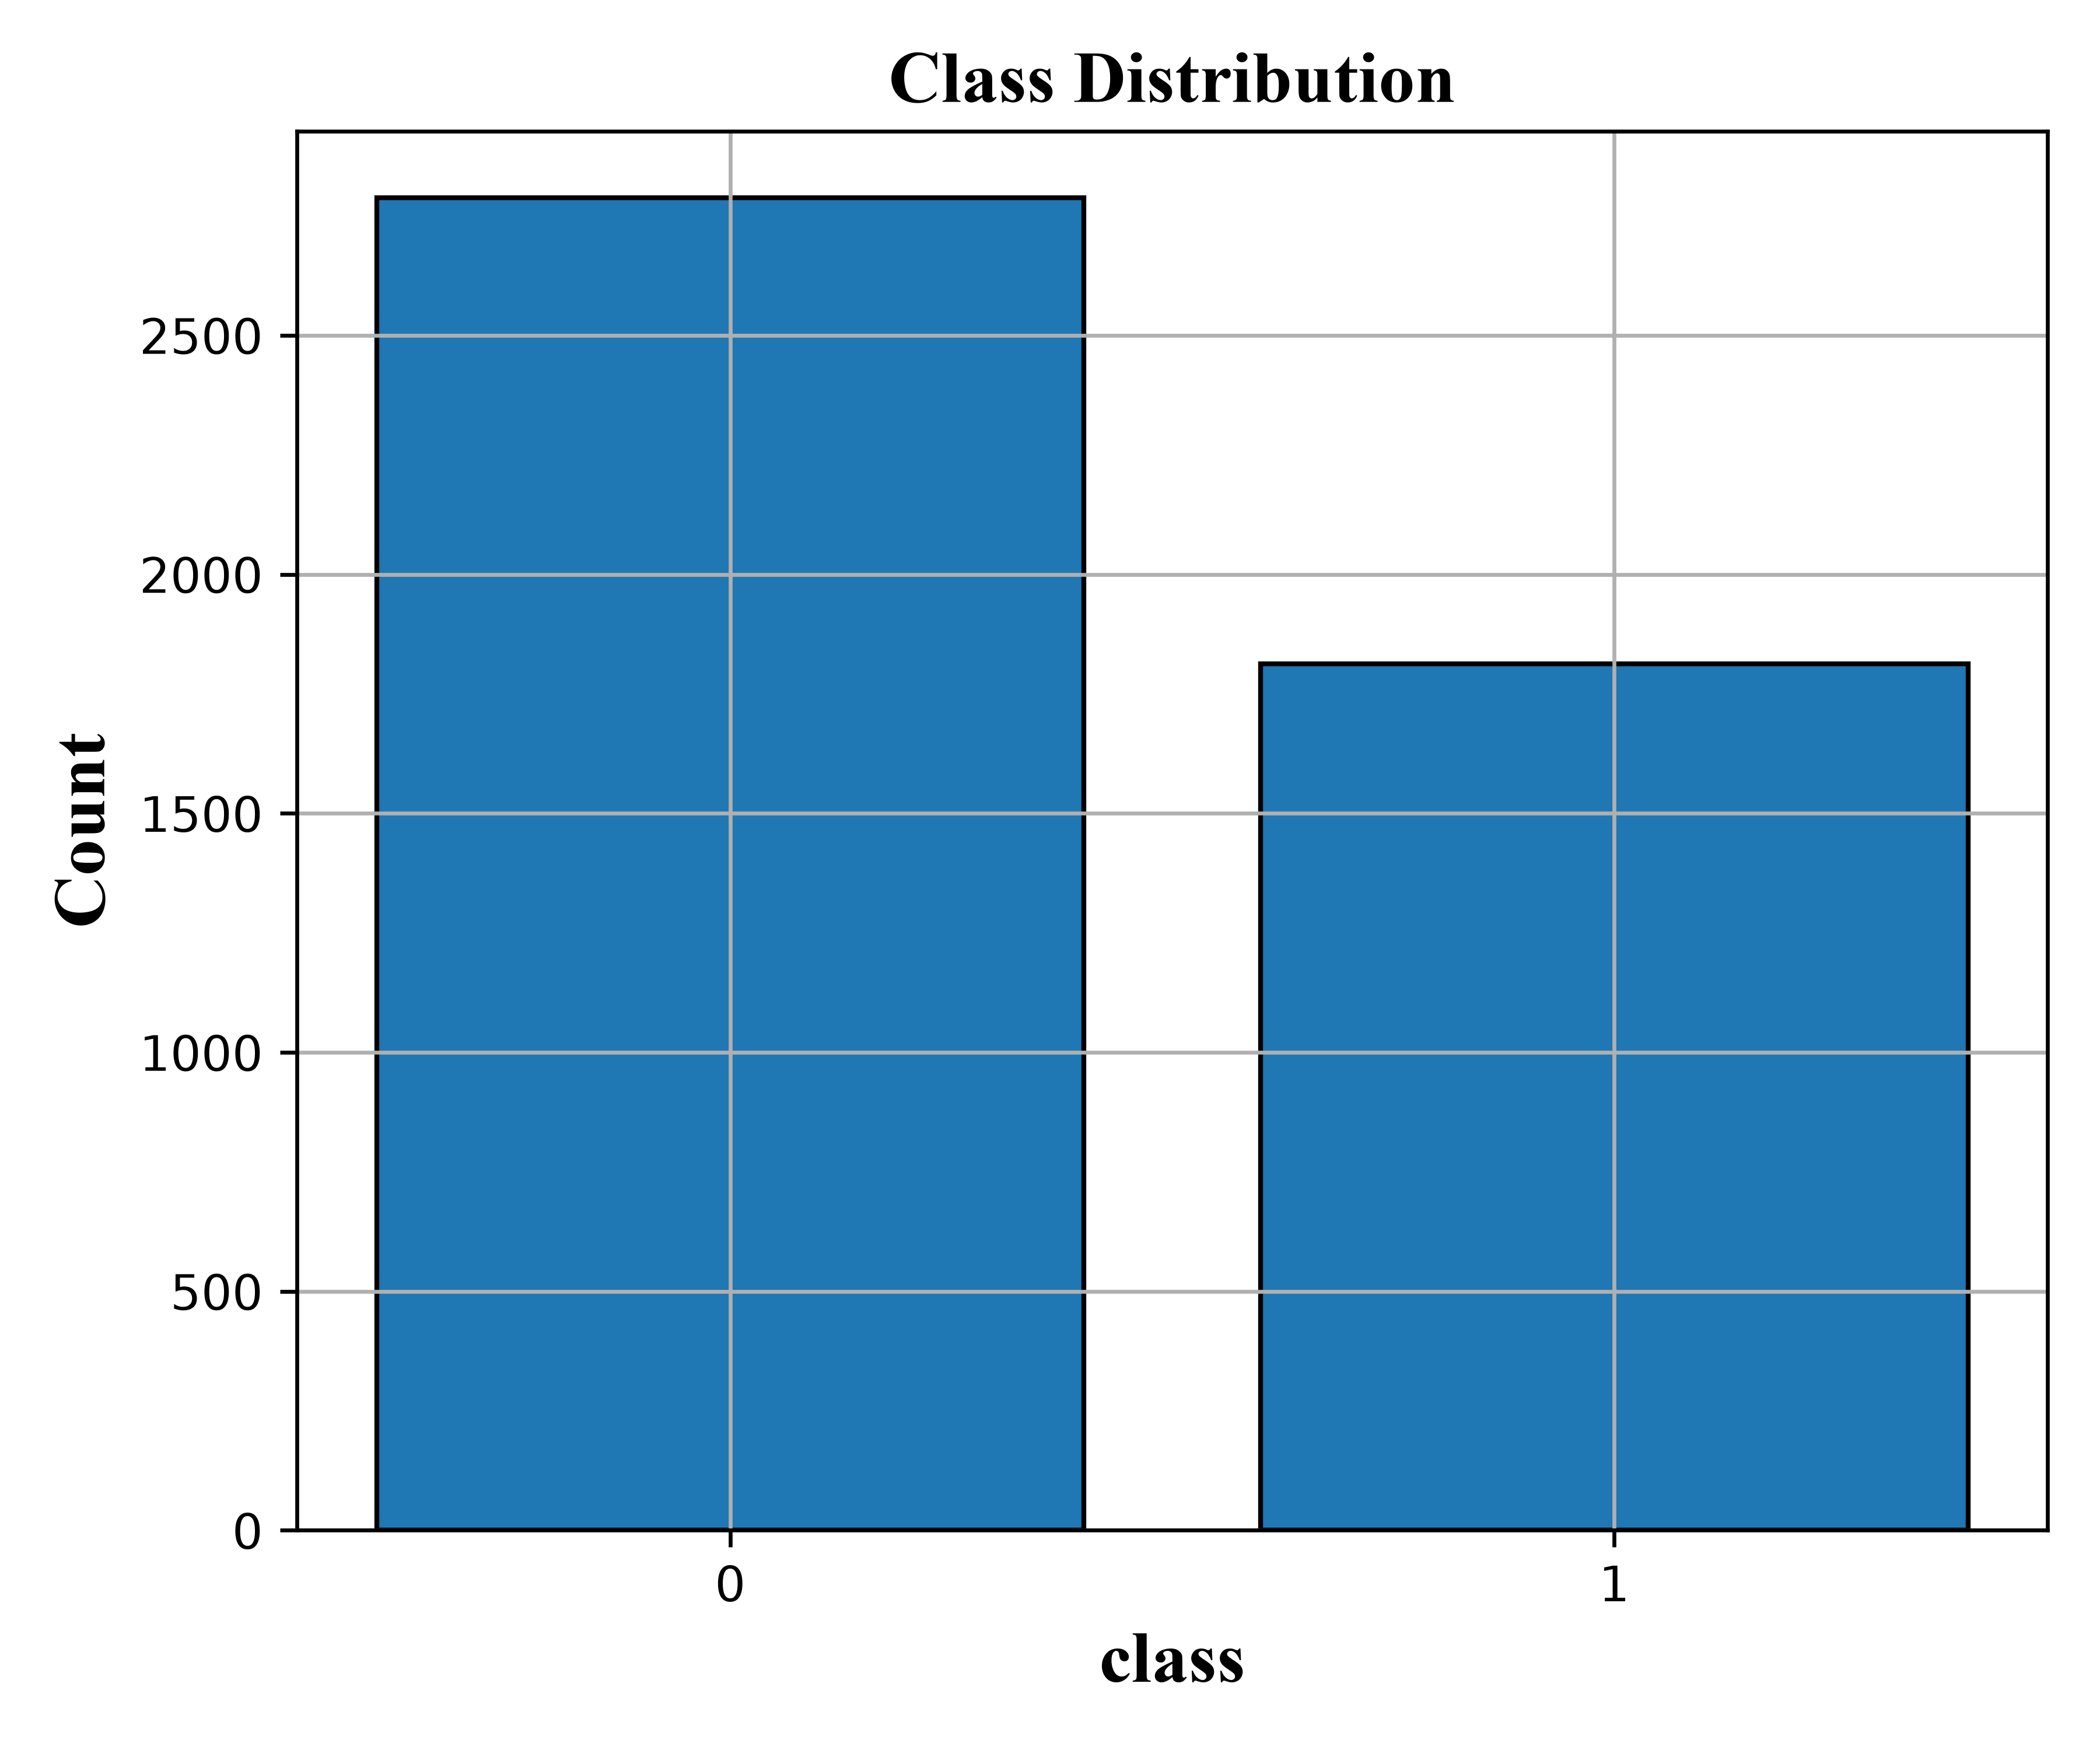
\includegraphics[width=0.6\linewidth]{class_distribution.png}
\caption{Class Distribution -- Spam (1) vs Non-Spam (0)}
\end{figure}

\textbf{Inference:}

The class distribution plot confirms a moderate imbalance, with approximately 60.6\% of emails labeled as non-spam and 39.4\% labeled as spam. This imbalance is not severe enough to require techniques such as SMOTE or class-weighting, but it does mean that accuracy alone can be slightly optimistic; therefore Precision, Recall, and F1-Score were also reported for both models to give a fuller picture of performance on the minority (spam) class.

\subsection{Correlation Analysis}

The correlation matrix was generated using all numerical features to identify their linear relationship with the target class.

\begin{figure}[H]
\centering
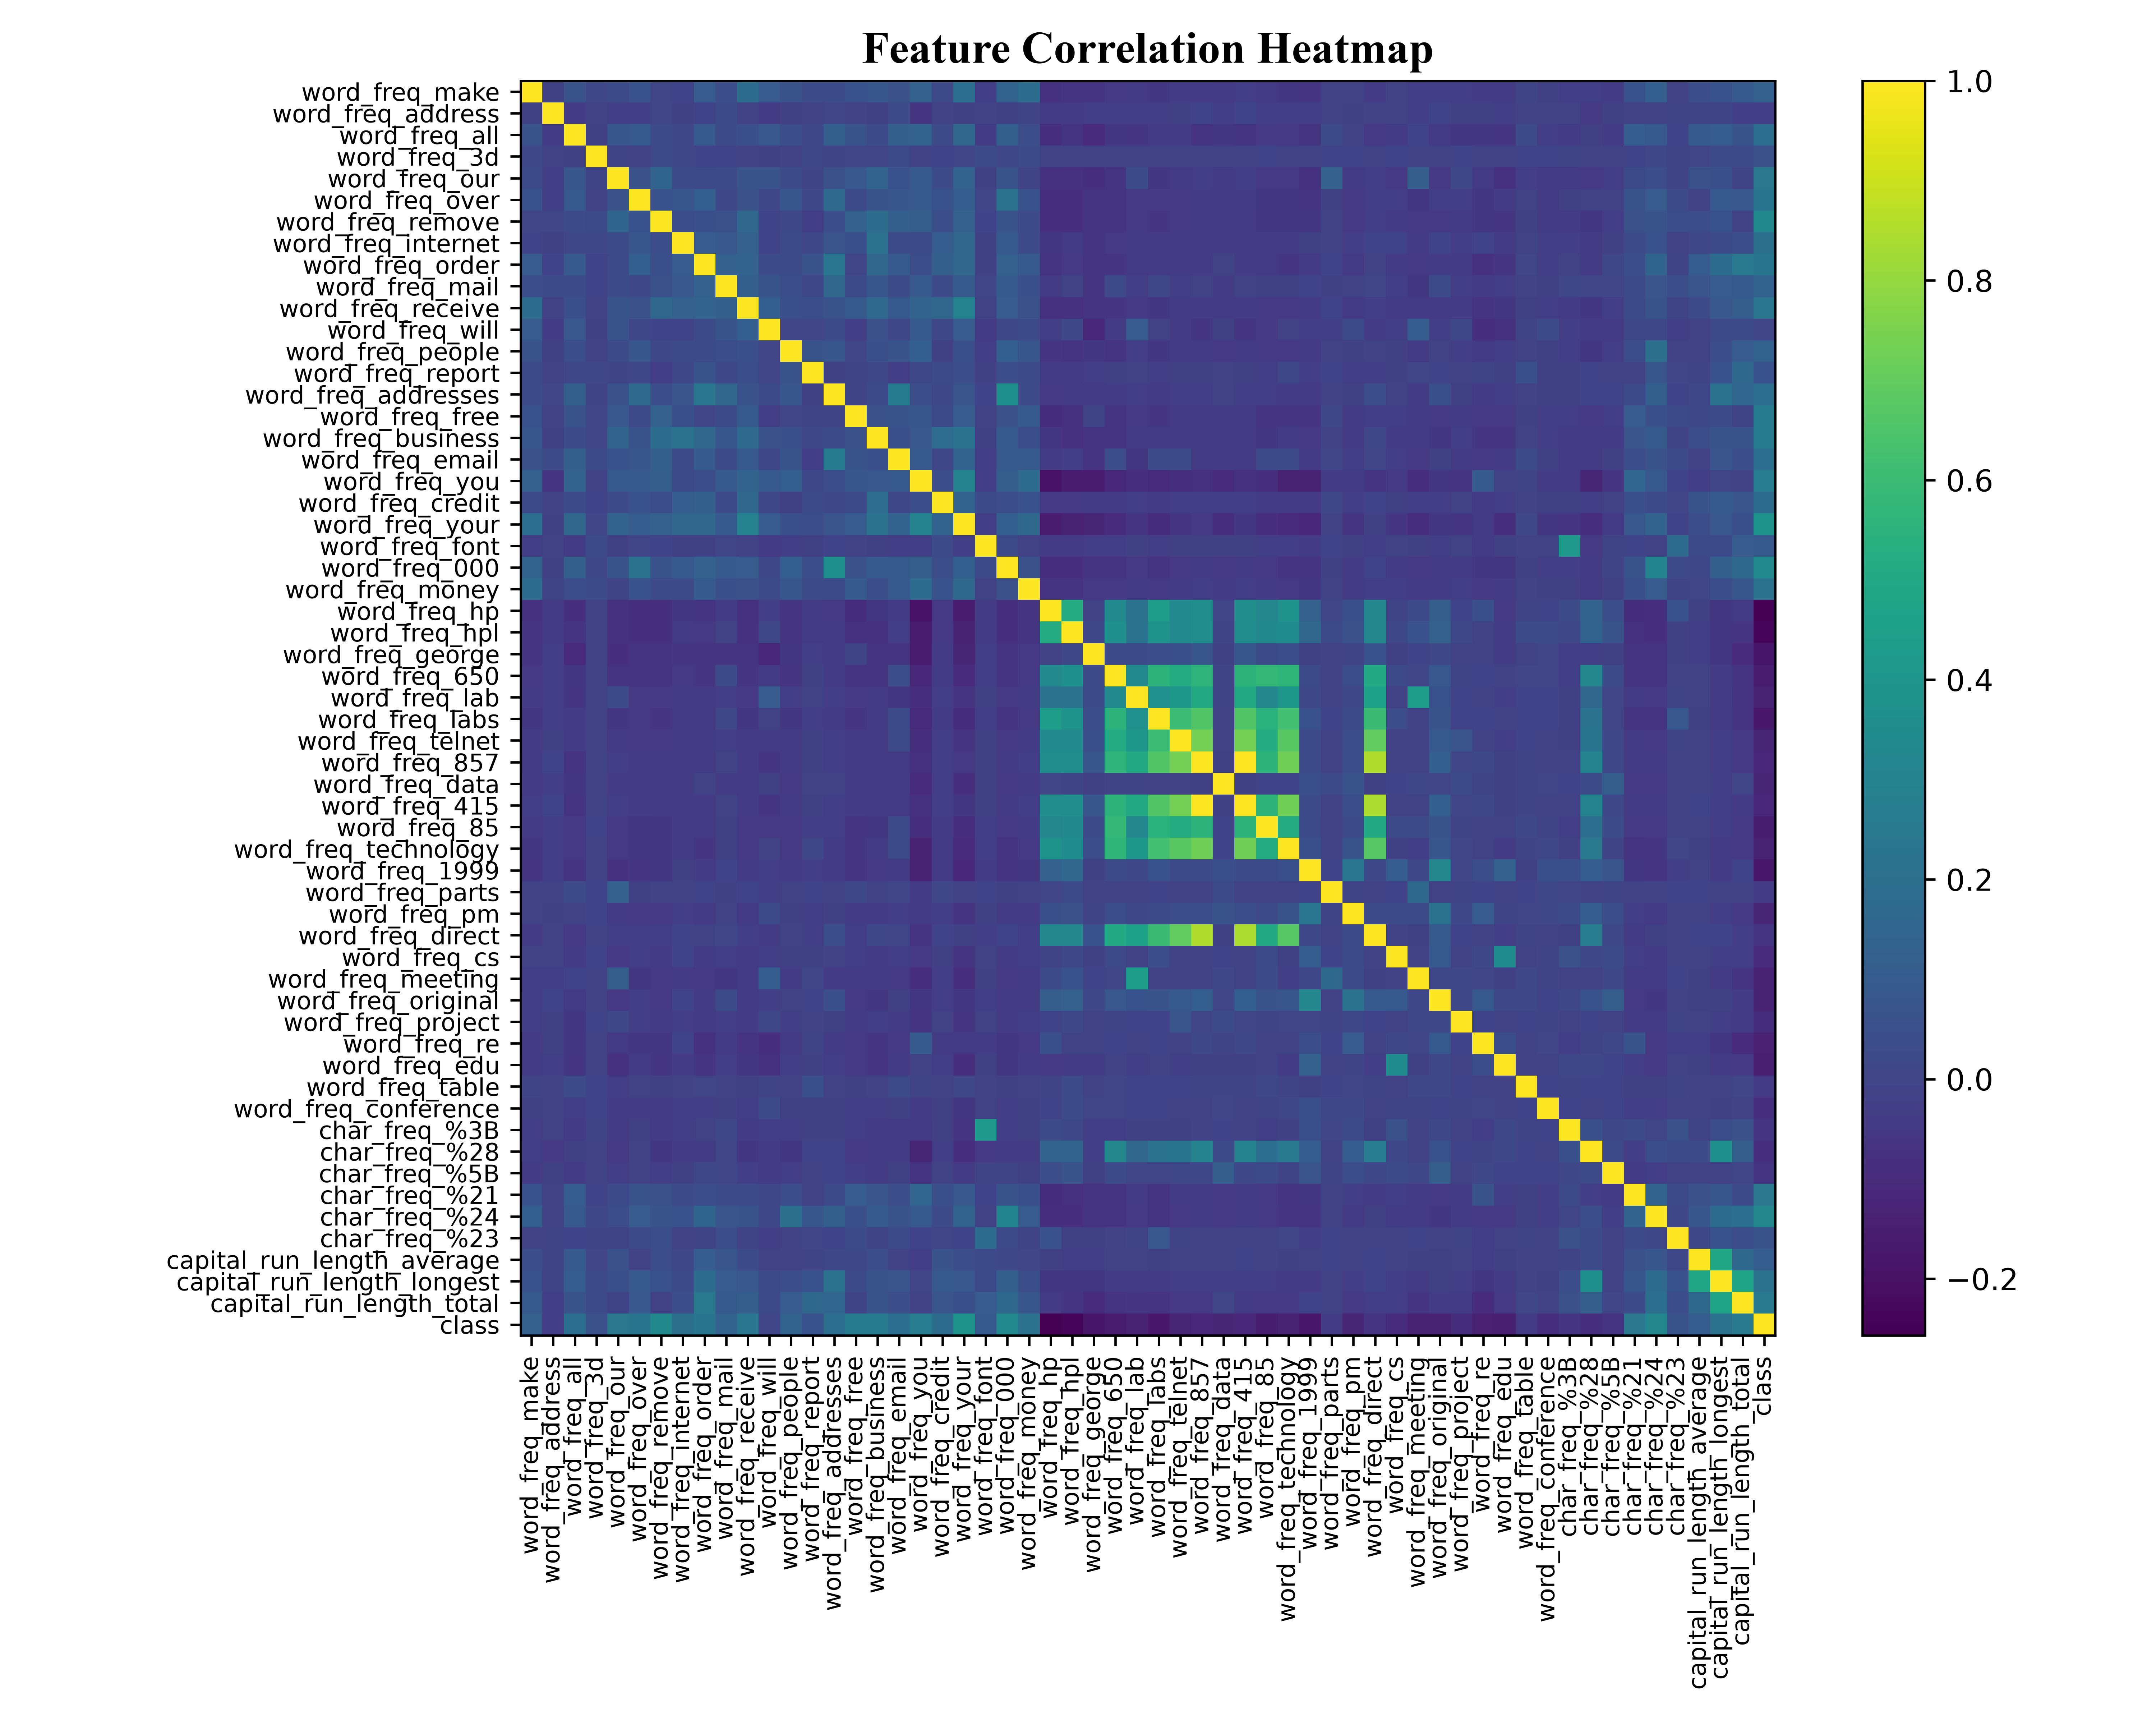
\includegraphics[width=0.7\linewidth]{correlation_heatmap.png}
\caption{Correlation Heatmap of Numerical Features}
\end{figure}

\begin{table}[H]
\centering
\begin{tabular}{lc}
\toprule
Feature & Correlation with Class \\
\midrule
word\_freq\_your & 0.3832 \\
word\_freq\_000 & 0.3348 \\
word\_freq\_remove & 0.3321 \\
char\_freq\_\%24 (\$) & 0.3236 \\
word\_freq\_you & 0.2737 \\
word\_freq\_free & 0.2632 \\
word\_freq\_business & 0.2632 \\
capital\_run\_length\_total & 0.2492 \\
\midrule
word\_freq\_hp & -0.2567 \\
word\_freq\_hpl & -0.2330 \\
word\_freq\_george & -0.1834 \\
word\_freq\_1999 & -0.1780 \\
\bottomrule
\end{tabular}
\caption{Strongest Positive and Negative Correlations with Spam Class}
\end{table}

\textbf{Inference:}

Words such as ``your'', ``000'', ``remove'', and the dollar-sign character show the strongest positive correlation with the spam class, matching intuitive spam vocabulary (marketing language, opt-out instructions, monetary references). Conversely, words such as ``hp'', ``hpl'', and ``george'' show strong negative correlation, which is explained by the dataset's origin -- it was collected from Hewlett-Packard (HP) Labs email accounts, so these terms are strong indicators of legitimate internal correspondence rather than spam. This confirms that the dataset contains strong, interpretable, and non-trivial linear signal suitable for both linear (Logistic Regression) and margin-based (SVM) classifiers.

\section{Data Preprocessing}

Data preprocessing for this experiment was comparatively lightweight, since the Spambase dataset contains no categorical columns and no missing values.

\subsection{Missing Value Handling}

No missing values were present in any of the 58 columns, so no imputation was required.

\subsection{Feature Scaling}

All 57 numerical features were standardized using \texttt{StandardScaler}:
\[
X_{scaled} = \frac{X-\mu}{\sigma}
\]
where $\mu$ is the feature mean and $\sigma$ is the feature standard deviation. Scaling is particularly important for this experiment because both Logistic Regression (regularization penalty) and SVM (margin/kernel computations) are sensitive to feature magnitude; without scaling, features with naturally larger ranges (e.g. \texttt{capital\_run\_length\_total}, which reaches values over 15000) would dominate the decision boundary relative to word frequency features bounded between 0 and roughly 20.

\subsection{Train-Test Split}

The processed dataset was divided into training and testing sets using an 80/20 split with \texttt{random\_state=42} for reproducibility.

\begin{table}[H]
\centering
\begin{tabular}{lc}
\toprule
Dataset & Samples \\
\midrule
Training Data & 3368 \\
Testing Data & 842 \\
\bottomrule
\end{tabular}
\caption{Train-Test Dataset Distribution}
\end{table}

The preprocessing pipeline produced $X_{train} = (3368, 57)$ and $X_{test} = (842, 57)$, with all 57 original features retained (no encoding-driven feature expansion was needed, unlike in the regression experiment).

\section{Implementation Details}

The implementation was modularized using reusable functions organized into dedicated source modules (\texttt{preprocessing.py}, \texttt{classification.py}, \texttt{hyperparameter.py}, \texttt{metrics.py}, \texttt{validation.py}, \texttt{timing.py}, \texttt{visualization.py}, \texttt{eda.py}):

\begin{itemize}
\item \texttt{perform\_classification\_eda()} -- runs the complete exploratory analysis and generates the consolidated 12-subplot EDA summary figure.
\item \texttt{preprocess\_data()} -- applies scaling and performs the train/test split.
\item \texttt{train\_classification()} -- trains a specified classification algorithm with given hyperparameters.
\item \texttt{grid\_search()} / \texttt{randomized\_search()} -- performs hyperparameter optimization via GridSearchCV or RandomizedSearchCV.
\item \texttt{classification\_metrics()} -- computes Accuracy, Precision, Recall, and F1-Score for a single model.
\item \texttt{compare\_classification\_models()} -- computes and tabulates metrics across multiple models.
\item \texttt{compare\_classification\_cross\_validation()} -- performs 5-fold cross-validation and reports per-fold and average accuracy.
\item \texttt{compare\_training\_prediction\_time()} -- benchmarks training and prediction runtime for each model.
\item \texttt{plot\_confusion\_matrix()}, \texttt{plot\_roc\_curve()}, \texttt{plot\_classification\_scores()}, \texttt{plot\_classification\_cv\_scores()} -- generate all required result visualizations.
\end{itemize}

This modular design mirrors the structure used in the regression experiment, allowing EDA, preprocessing, training, tuning, and evaluation logic to be reused with minimal changes.

\section{Machine Learning Algorithm}

Two classification paradigms are implemented and compared in this experiment: Logistic Regression, a linear probabilistic classifier, and Support Vector Machines, a margin-based classifier capable of both linear and non-linear (kernelized) decision boundaries.

\subsection{Logistic Regression}

Logistic Regression models the probability that a given sample belongs to the positive class using the sigmoid (logistic) function applied to a linear combination of features:
\[
P(y=1\mid x) = \sigma(z) = \frac{1}{1+e^{-z}}, \qquad z = \beta_0 + \beta_1 x_1 + \beta_2 x_2 + \dots + \beta_n x_n
\]

The model is trained by minimizing the (regularized) log-loss:
\[
Loss = -\frac{1}{n}\sum_{i=1}^{n}\Big[y_i \log(\hat{p}_i) + (1-y_i)\log(1-\hat{p}_i)\Big] + \frac{1}{C}\,R(\beta)
\]
where $\hat{p}_i$ is the predicted probability, $C$ is the inverse regularization strength, and $R(\beta)$ is either an L1 penalty ($\sum|\beta_j|$) or an L2 penalty ($\sum \beta_j^2$) depending on the chosen \texttt{penalty} hyperparameter.

\textbf{Advantages:} Computationally efficient; produces well-calibrated probability estimates; highly interpretable coefficients; L1 penalty enables automatic feature selection.

\textbf{Limitations:} Assumes a linear decision boundary in the (transformed) feature space; can underperform on datasets with strongly non-linear class boundaries; sensitive to feature scaling.

\subsection{Support Vector Machine (SVM)}

Support Vector Machines find the hyperplane that maximizes the margin between classes. For a linearly separable case, the decision function is:
\[
f(x) = w^T x + b
\]
where the optimization problem seeks to maximize the margin $\frac{2}{\|w\|}$ subject to correct classification of all (or most, under the soft-margin formulation) training points. The soft-margin formulation introduces a penalty parameter $C$ that trades off margin width against misclassification of training points:
\[
\min_{w,b,\xi} \; \frac{1}{2}\|w\|^2 + C\sum_{i=1}^{n}\xi_i \quad \text{subject to} \quad y_i(w^Tx_i+b) \geq 1-\xi_i,\ \xi_i \geq 0
\]

For non-linear boundaries, SVM uses the \textbf{kernel trick} to implicitly map inputs into a higher-dimensional space without explicitly computing the transformation:
\begin{itemize}
\item \textbf{Linear kernel:} $K(x_i,x_j) = x_i^T x_j$
\item \textbf{Polynomial kernel:} $K(x_i,x_j) = (\gamma\, x_i^T x_j + r)^d$
\item \textbf{RBF (Gaussian) kernel:} $K(x_i,x_j) = \exp(-\gamma\|x_i-x_j\|^2)$
\item \textbf{Sigmoid kernel:} $K(x_i,x_j) = \tanh(\gamma\, x_i^T x_j + r)$
\end{itemize}

\textbf{Advantages:} Effective in high-dimensional feature spaces; kernel trick allows modeling of complex, non-linear decision boundaries; robust to overfitting when the margin is well-regularized via $C$.

\textbf{Limitations:} Computationally expensive to train on larger datasets; performance is highly sensitive to the choice of kernel, $C$, and $\gamma$; less directly interpretable than Logistic Regression; does not natively output probabilities (requires an additional Platt-scaling step, i.e. \texttt{probability=True}).

\section{Experimental Setup}

\begin{table}[H]
\centering
\begin{tabular}{ll}
\toprule
Parameter & Details \\
\midrule
Programming Language & Python \\
Machine Learning Library & Scikit-Learn \\
Data Processing Library & Pandas, NumPy \\
Visualization Library & Matplotlib \\
Development Environment & Jupyter Notebook \\
Python Version & Python 3.x (Anaconda Environment) \\
Operating System & Linux (Anaconda Environment) \\
Dataset Size & 4601 samples \\
Processor & Intel-based system \\
\bottomrule
\end{tabular}
\caption{Experimental Environment}
\end{table}

\section{Hyperparameter Selection}

GridSearchCV with 5-fold cross-validation, scored on accuracy, was used to tune both Logistic Regression and SVM.

\subsection*{Logistic Regression Search Space}

\begin{table}[H]
\centering
\begin{tabular}{ll}
\toprule
Parameter & Search Space \\
\midrule
Penalty & $\{$L1, L2$\}$ \\
$C$ & $\{0.01, 0.1, 1, 10, 100\}$ \\
Solver & $\{$liblinear, saga$\}$ \\
\bottomrule
\end{tabular}
\caption{Logistic Regression Hyperparameter Search Space}
\end{table}

\begin{table}[H]
\centering
\begin{tabular}{ll}
\toprule
Parameter & Best Value \\
\midrule
$C$ & 100 \\
Penalty & L1 \\
Solver & saga \\
Best CV Accuracy & 0.9231 \\
\bottomrule
\end{tabular}
\caption{Best Logistic Regression Hyperparameters}
\end{table}

\subsection*{SVM Search Space}

\begin{table}[H]
\centering
\begin{tabular}{ll}
\toprule
Parameter & Search Space \\
\midrule
Kernel & $\{$linear, poly, rbf, sigmoid$\}$ \\
$C$ & $\{0.1, 1, 10, 100\}$ \\
$\gamma$ & $\{$scale, auto$\}$ (rbf, sigmoid, poly) \\
Degree & $\{2, 3, 4\}$ (poly only) \\
\bottomrule
\end{tabular}
\caption{SVM Hyperparameter Search Space}
\end{table}

\begin{table}[H]
\centering
\begin{tabular}{ll}
\toprule
Parameter & Best Value \\
\midrule
Kernel & RBF \\
$C$ & 10 \\
$\gamma$ & scale \\
Best CV Accuracy & 0.9299 \\
\bottomrule
\end{tabular}
\caption{Best SVM Hyperparameters}
\end{table}

\textbf{Inference:} Logistic Regression selected the strongest permissible $C$ (100, i.e. weakest regularization) combined with an L1 penalty, suggesting that most of the 57 features carry genuine signal and only a modest sparsity constraint was needed to prevent overfitting. SVM's selection of the RBF kernel over Linear, Polynomial, and Sigmoid indicates that a mild degree of non-linearity in the decision boundary improves classification, though the relatively modest gap between the linear kernel's baseline accuracy (92.16\%) and the tuned RBF's cross-validation accuracy (92.99\%) suggests the added non-linearity provides only marginal benefit over a well-regularized linear separator.

\section{Baseline Model Performance}

\subsection*{Baseline Logistic Regression (Untuned)}

\begin{table}[H]
\centering
\begin{tabular}{lc}
\toprule
Metric & Value \\
\midrule
Accuracy & 0.9145 \\
Precision & 0.9284 \\
Recall & 0.8663 \\
F1-Score & 0.8963 \\
\bottomrule
\end{tabular}
\caption{Baseline Logistic Regression Performance (Default Hyperparameters)}
\end{table}

\begin{figure}[H]
\centering
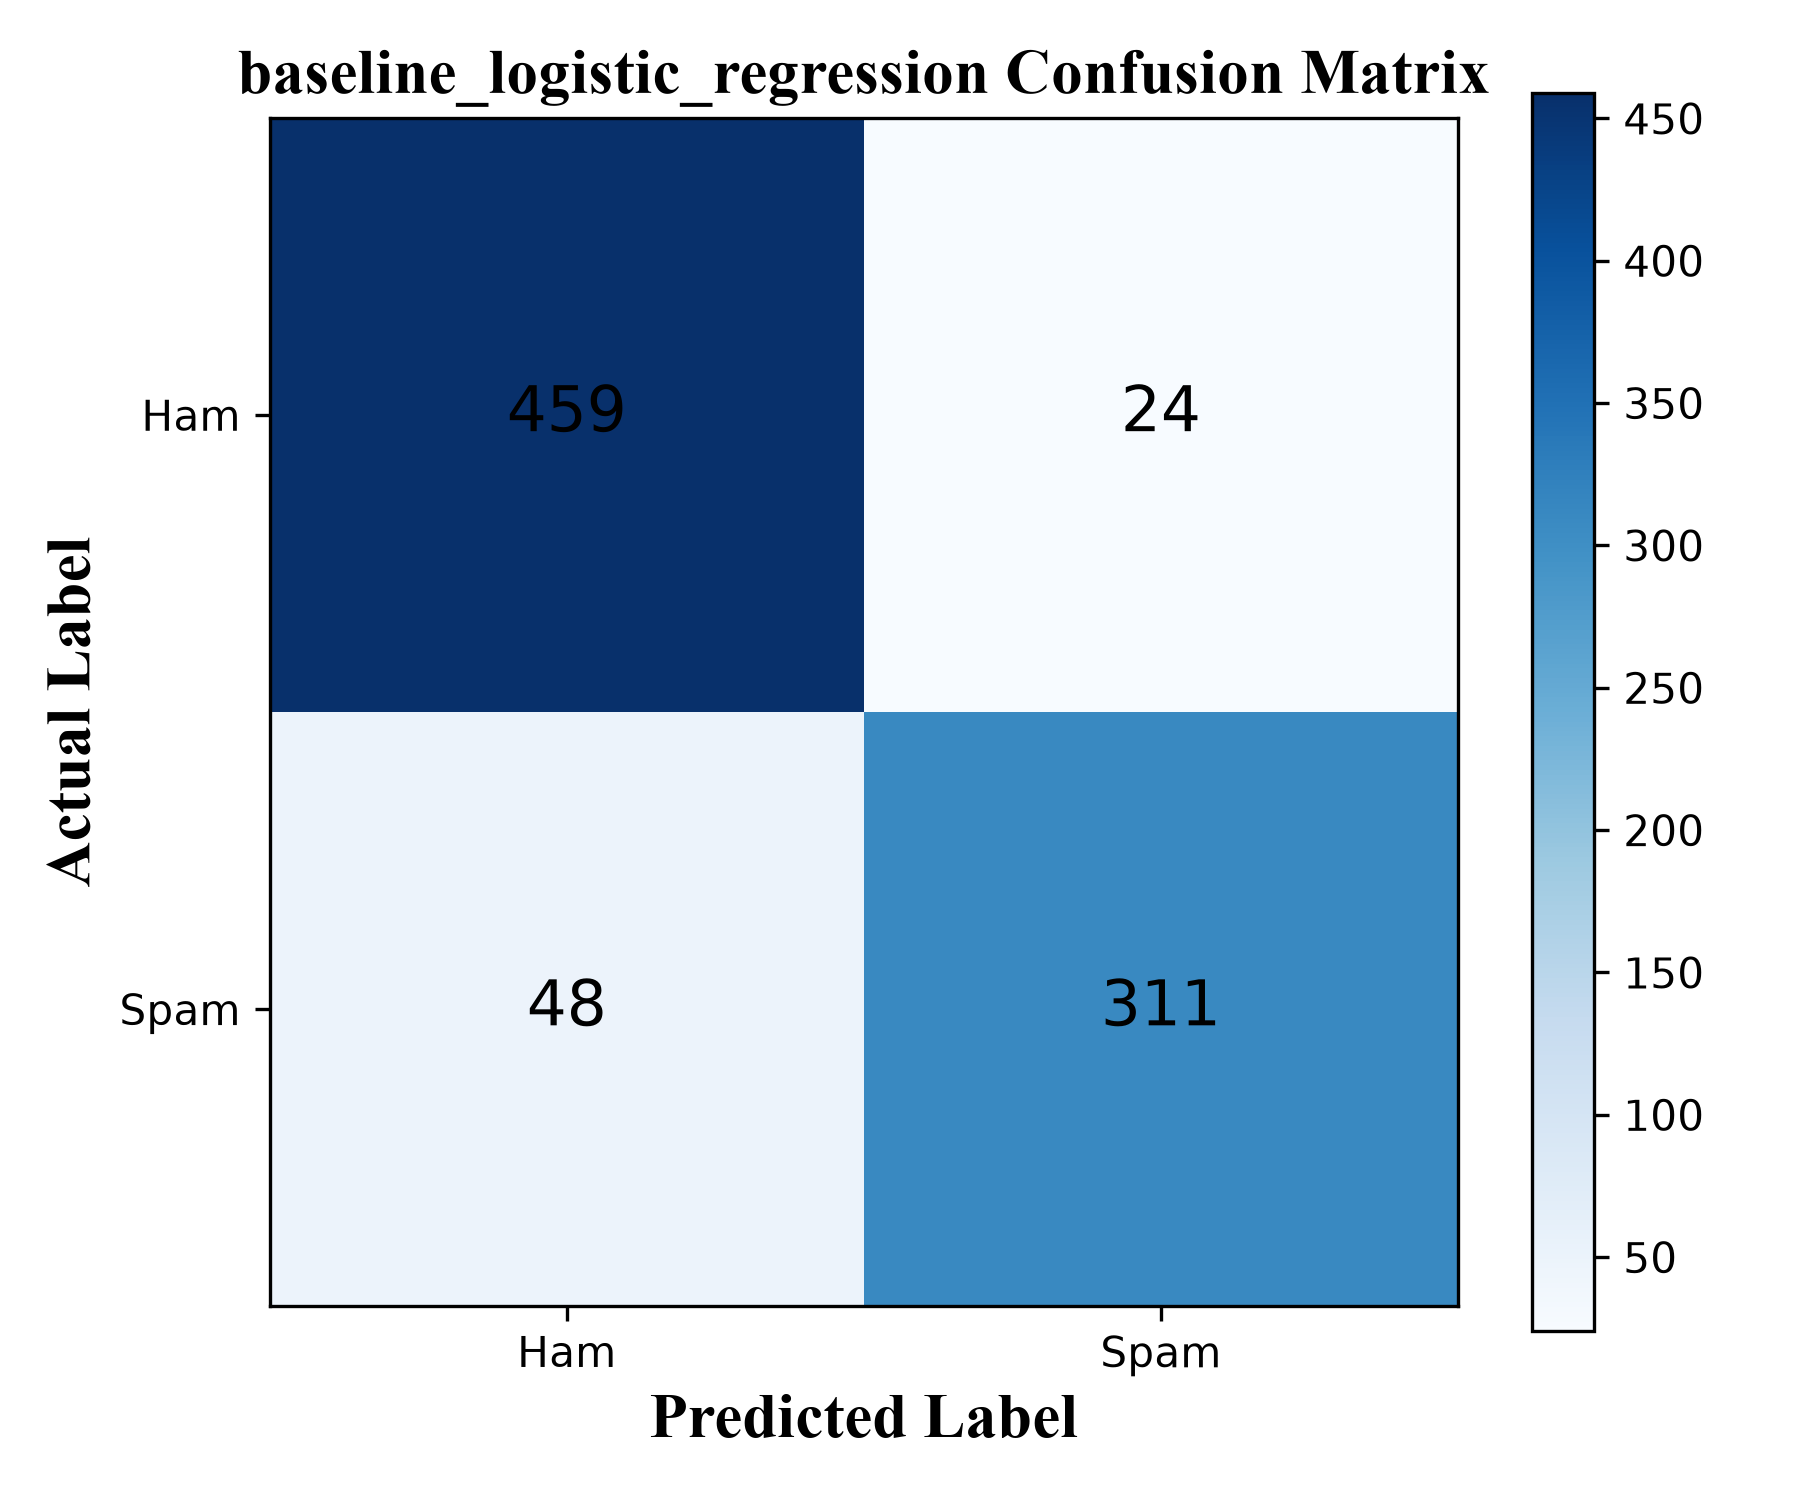
\includegraphics[width=0.55\linewidth]{baseline_logistic_regression_confusion_matrix.png}
\caption{Confusion Matrix -- Baseline Logistic Regression}
\end{figure}

\textbf{Inference:} The baseline Logistic Regression model, trained with default hyperparameters, already achieves a strong accuracy of 91.45\%. The confusion matrix shows relatively few false positives but a comparatively higher number of false negatives (missed spam), reflected in the lower recall (0.8663) compared to precision (0.9284), indicating the untuned model is slightly conservative about labeling an email as spam.

\subsection*{SVM Kernel-wise Baseline Comparison}

Four SVM kernels were trained with default hyperparameters to compare baseline kernel behavior prior to tuning.

\begin{table}[H]
\centering
\begin{tabular}{lcc}
\toprule
Kernel & Accuracy & F1-Score \\
\midrule
Linear & 0.9216 & 0.9060 \\
Polynomial & 0.7613 & 0.6257 \\
RBF & 0.9181 & 0.9013 \\
Sigmoid & 0.8777 & 0.8543 \\
\bottomrule
\end{tabular}
\caption{Baseline SVM Kernel Comparison (Default Hyperparameters)}
\end{table}

\begin{table}[H]
\centering
\begin{tabular}{lrr}
\toprule
Kernel & Training Time (s) & Prediction Time (s) \\
\midrule
Sigmoid & 0.7801 & 0.0269 \\
Polynomial & 1.1921 & 0.0341 \\
RBF & 1.2333 & 0.1159 \\
Linear & 1.2761 & 0.0128 \\
\bottomrule
\end{tabular}
\caption{Baseline SVM Kernel Training and Prediction Time}
\end{table}

\begin{figure}[H]
\centering
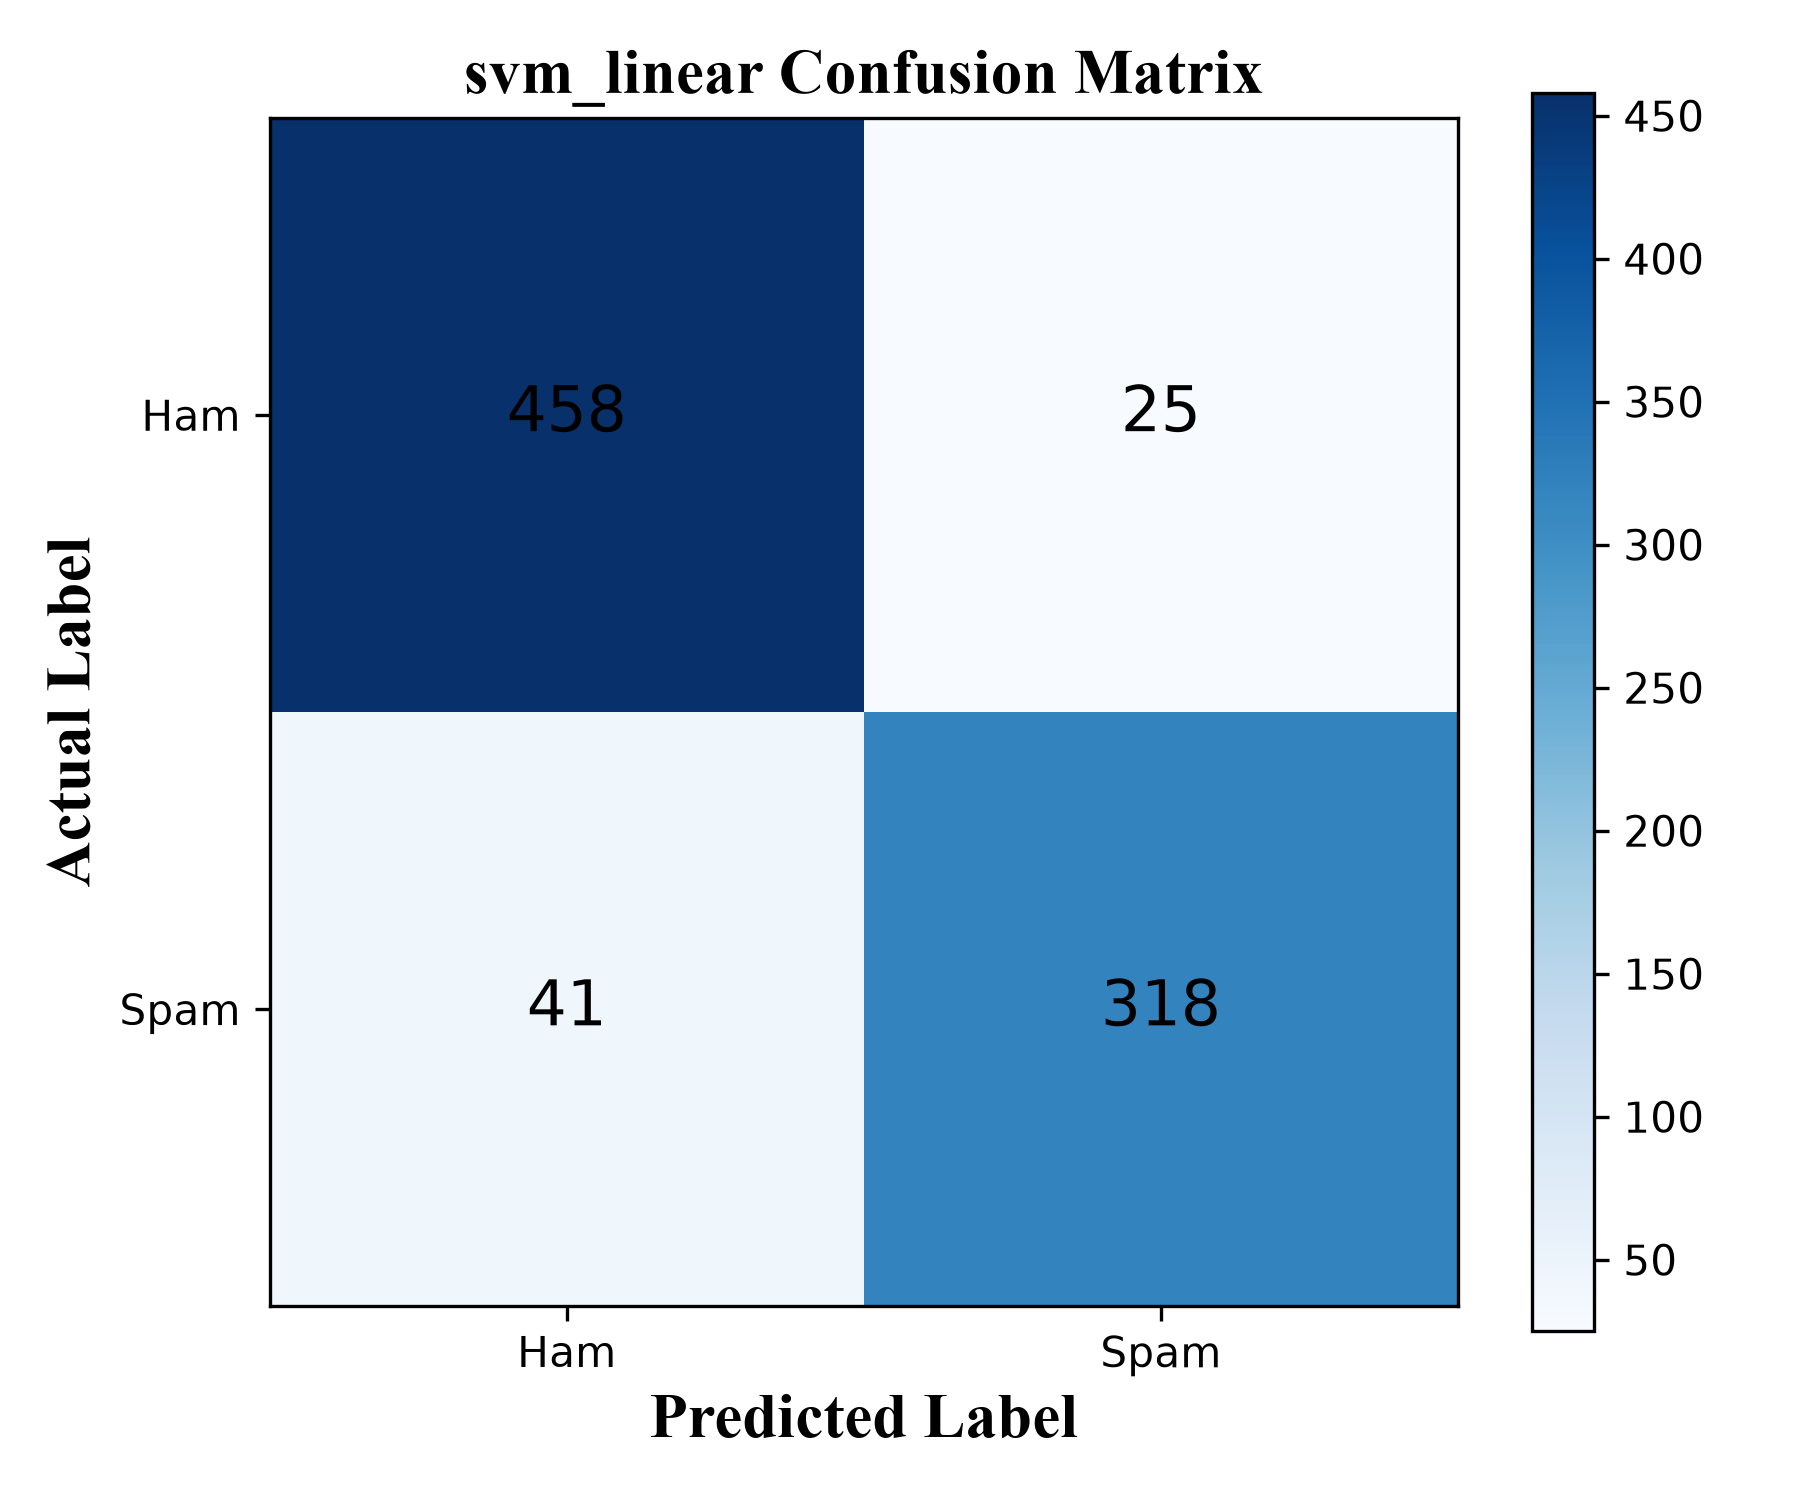
\includegraphics[width=0.55\linewidth]{svm_linear_confusion_matrix.png}
\caption{Confusion Matrix -- SVM (Linear Kernel, Default Parameters)}
\end{figure}

\begin{figure}[H]
\centering
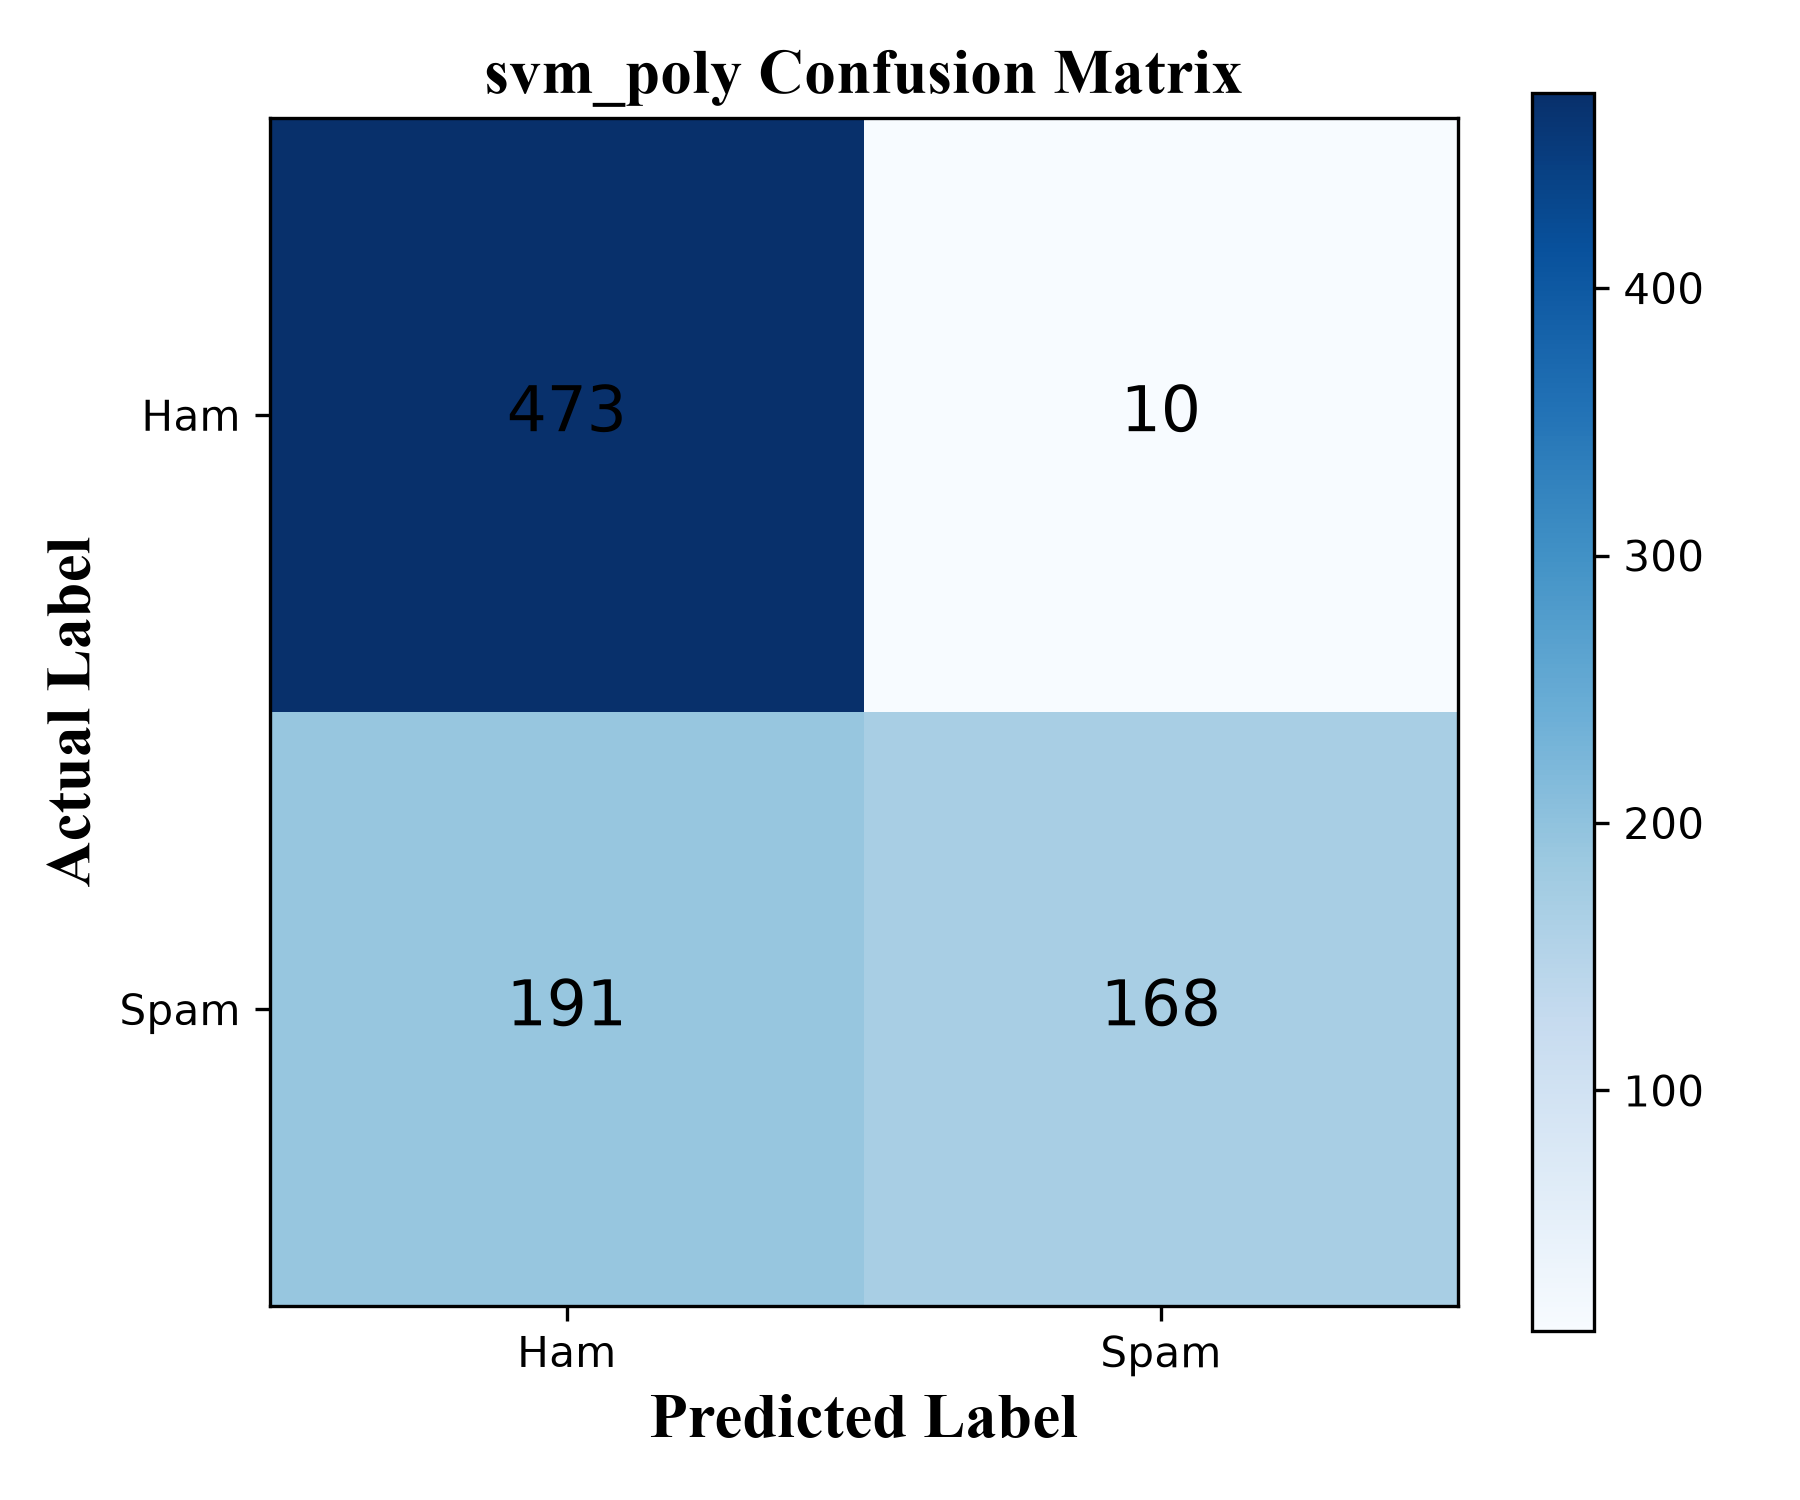
\includegraphics[width=0.55\linewidth]{svm_poly_confusion_matrix.png}
\caption{Confusion Matrix -- SVM (Polynomial Kernel, Default Parameters)}
\end{figure}

\begin{figure}[H]
\centering
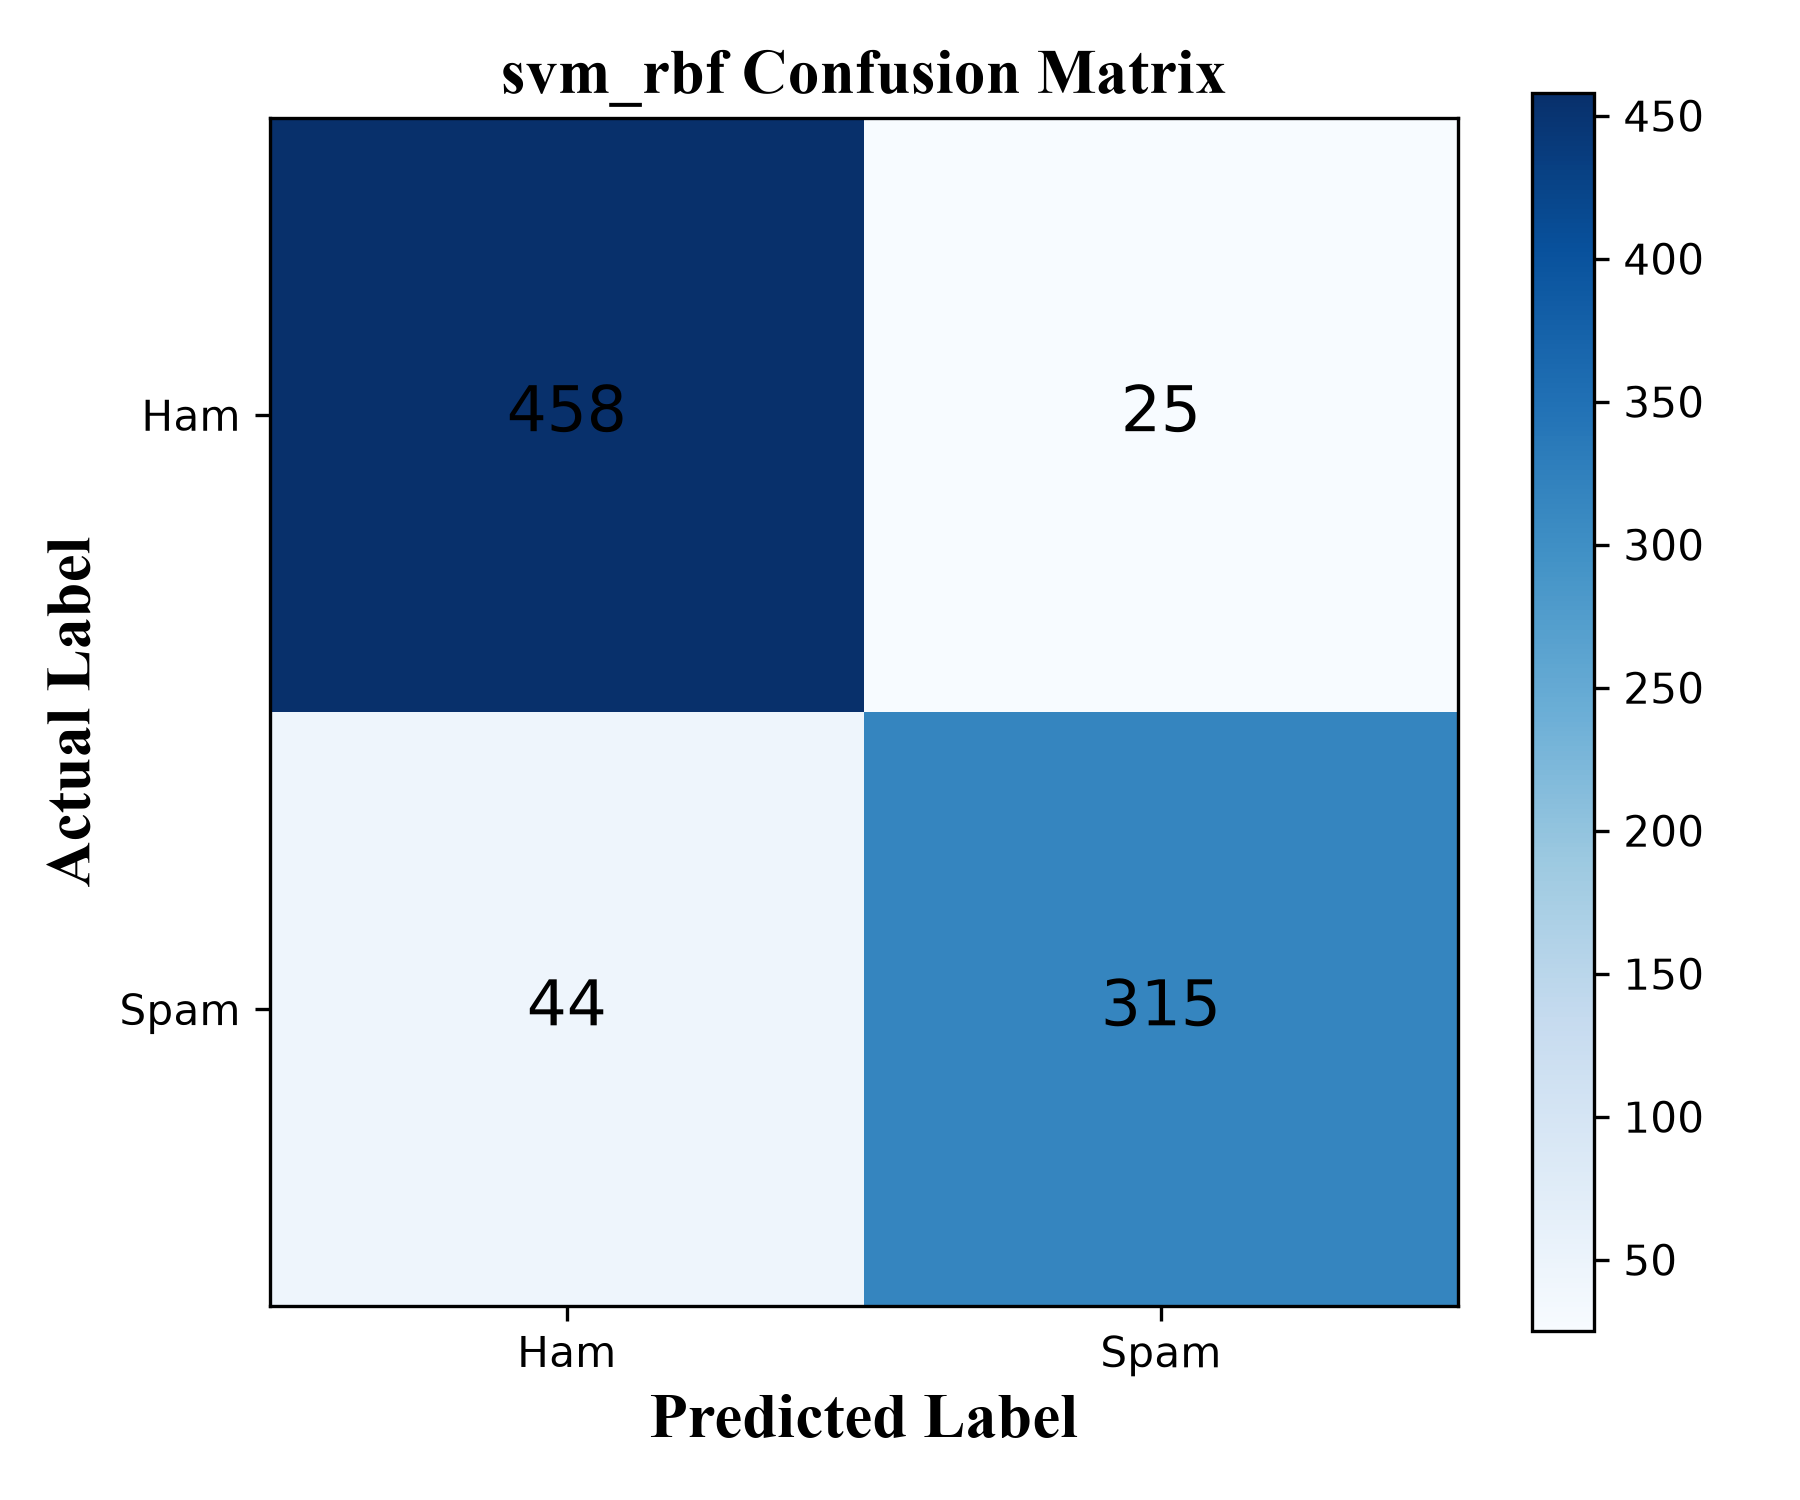
\includegraphics[width=0.55\linewidth]{svm_rbf_confusion_matrix.png}
\caption{Confusion Matrix -- SVM (RBF Kernel, Default Parameters)}
\end{figure}

\begin{figure}[H]
\centering
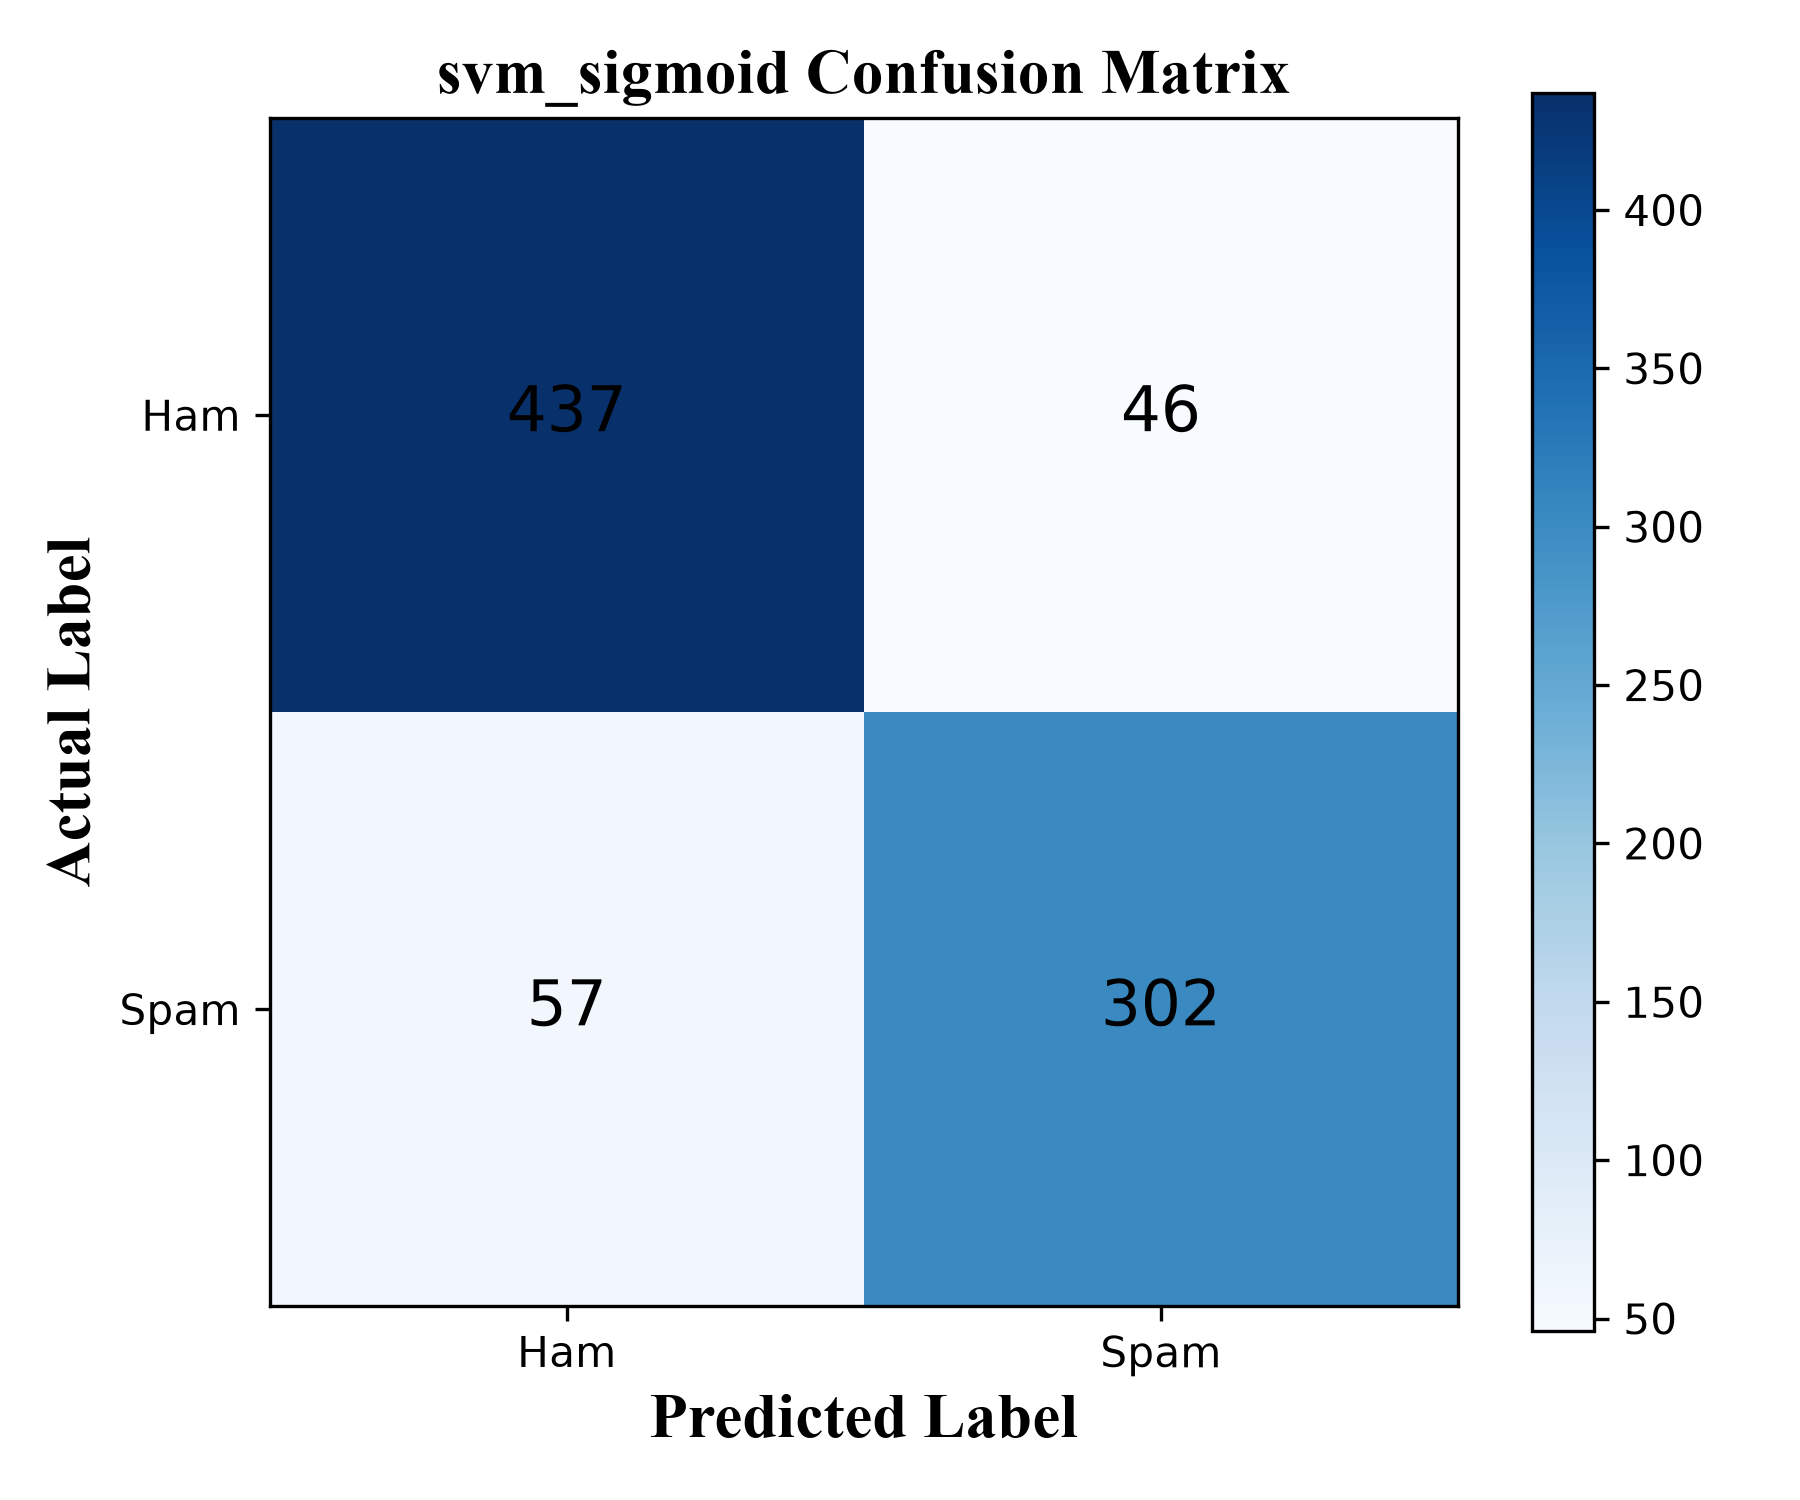
\includegraphics[width=0.55\linewidth]{svm_sigmoid_confusion_matrix.png}
\caption{Confusion Matrix -- SVM (Sigmoid Kernel, Default Parameters)}
\end{figure}

\textbf{Inference:} Among the four kernels at default settings, the Linear and RBF kernels perform strongly and almost identically (92.16\% and 91.81\% accuracy respectively), suggesting the underlying class boundary is close to linear in the scaled 57-dimensional feature space. The Polynomial kernel performs drastically worse (76.13\% accuracy, F1 = 0.6257) at default settings, most likely because the default degree (3) and unscaled coefficient term cause severe overfitting or underfitting artifacts without proper tuning of $\gamma$ and degree. The Sigmoid kernel performs moderately (87.77\%), consistent with its known sensitivity to hyperparameter choice and its structural similarity to a poorly calibrated neural activation function. Notably, the Sigmoid kernel is fastest to train while RBF has the highest prediction time due to its need to compute distances to all support vectors.

\section{Tuned Model Performance}

\subsection*{Tuned Logistic Regression}

\begin{table}[H]
\centering
\begin{tabular}{lc}
\toprule
Metric & Value \\
\midrule
Accuracy & 0.9204 \\
Precision & 0.9320 \\
Recall & 0.8774 \\
F1-Score & 0.9039 \\
\bottomrule
\end{tabular}
\caption{Tuned Logistic Regression Performance (Best Parameters: $C=100$, penalty = L1, solver = saga)}
\end{table}

\begin{figure}[H]
\centering
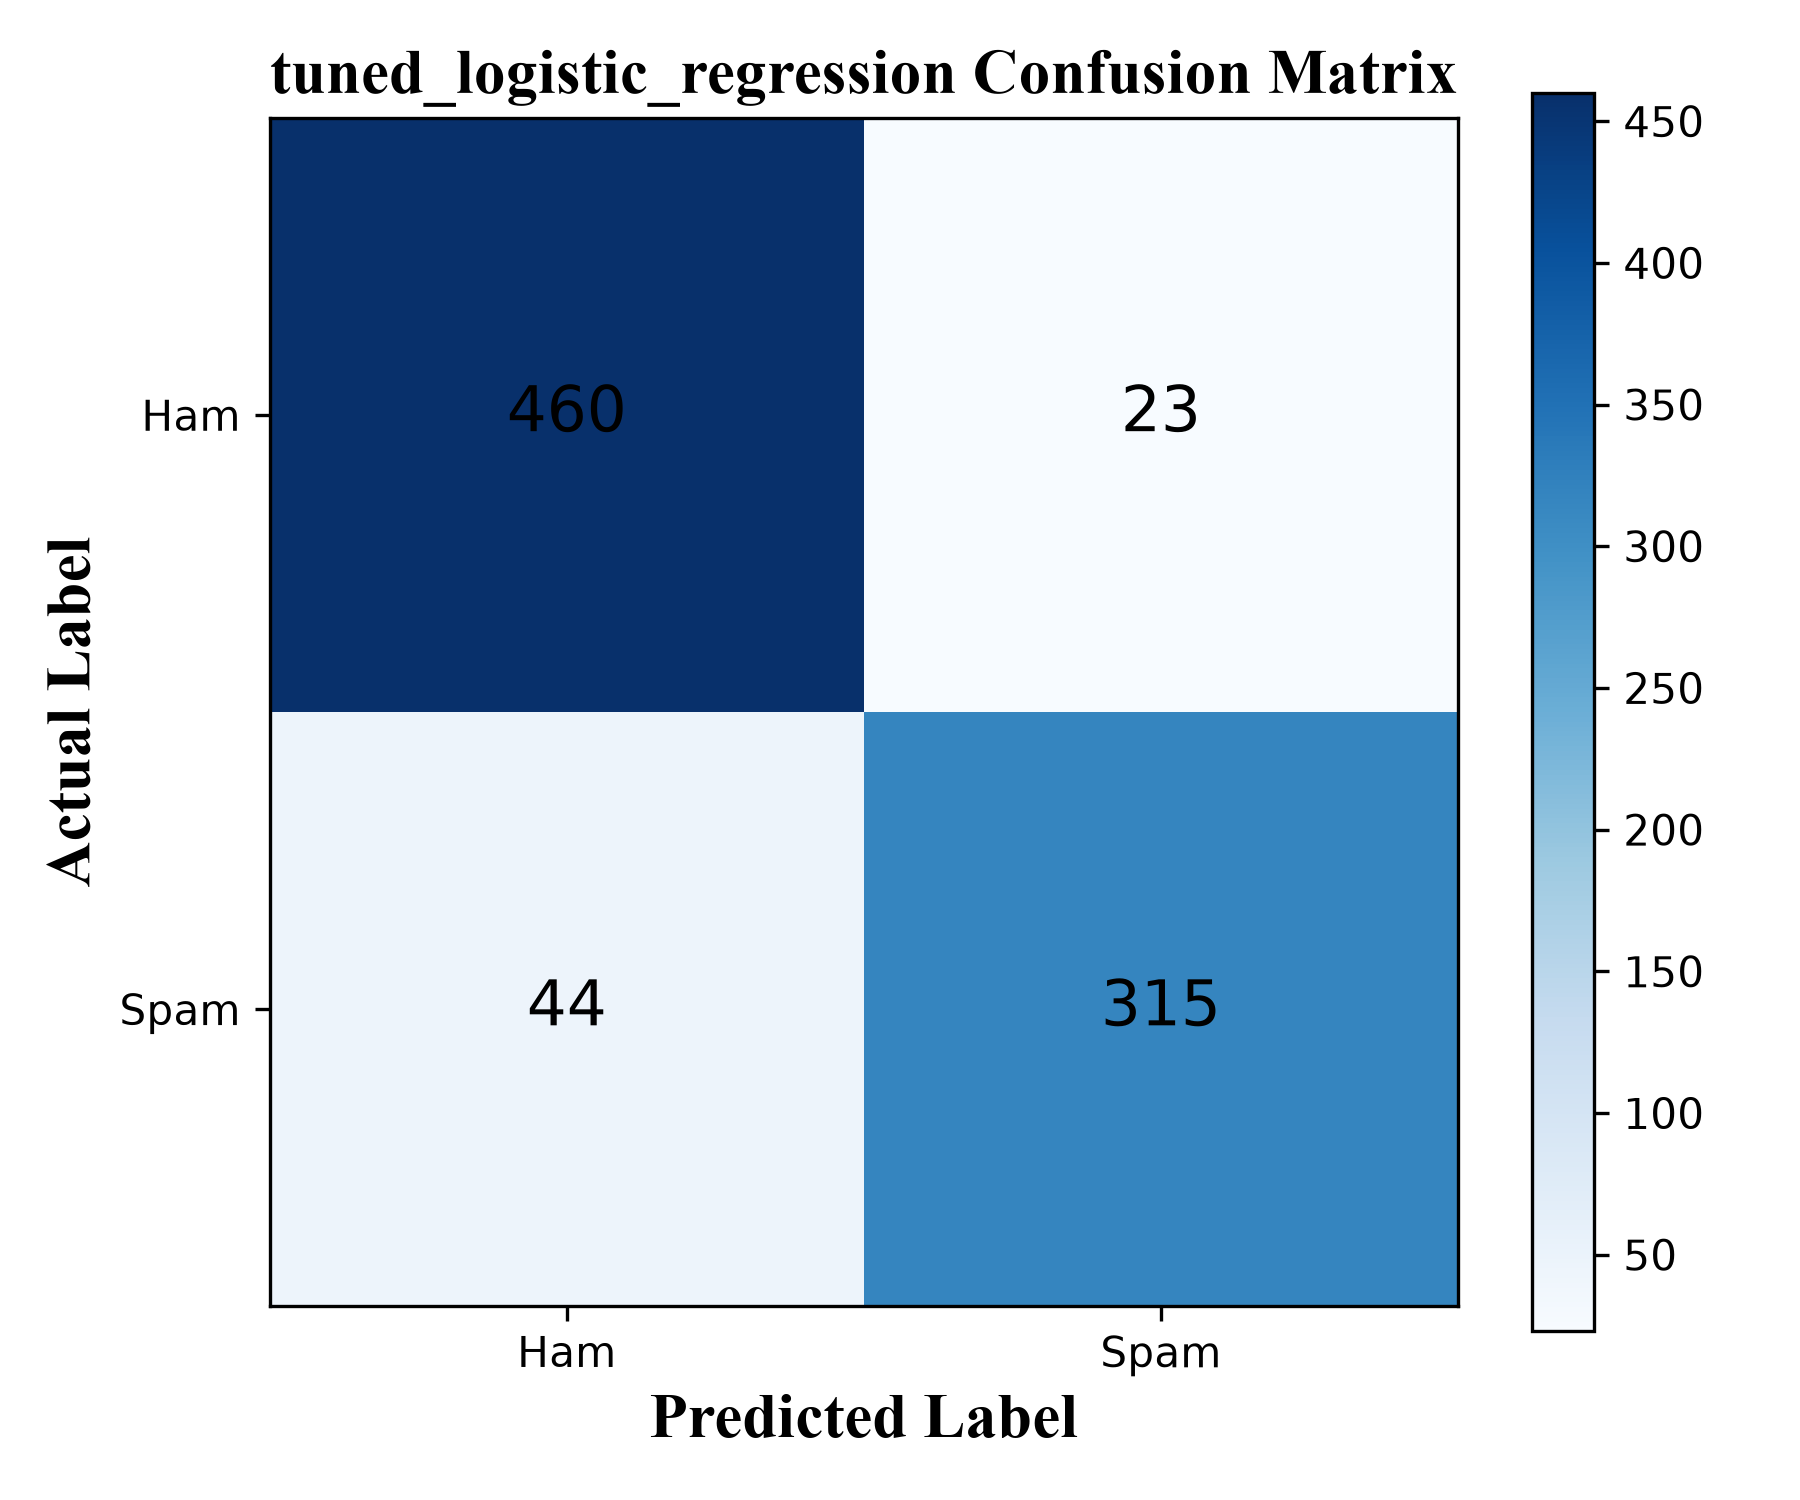
\includegraphics[width=0.55\linewidth]{tuned_logistic_regression_confusion_matrix.png}
\caption{Confusion Matrix -- Tuned Logistic Regression}
\end{figure}

\textbf{Inference:} Hyperparameter tuning improved Logistic Regression's test accuracy from 91.45\% to 92.04\% and F1-Score from 0.8963 to 0.9039. The improvement is driven primarily by an increase in recall (0.8663 $\to$ 0.8774), meaning the tuned model catches more true spam emails while maintaining (and slightly improving) precision. The L1 penalty additionally provides implicit feature selection, which can improve interpretability by zeroing out coefficients for less informative word/character frequencies.

\subsection*{Tuned SVM}

\begin{table}[H]
\centering
\begin{tabular}{lc}
\toprule
Metric & Value \\
\midrule
Accuracy & 0.9133 \\
Precision & 0.9206 \\
Recall & 0.8719 \\
F1-Score & 0.8956 \\
\bottomrule
\end{tabular}
\caption{Tuned SVM Performance (Best Parameters: kernel = RBF, $C=10$, $\gamma$ = scale)}
\end{table}

\begin{figure}[H]
\centering
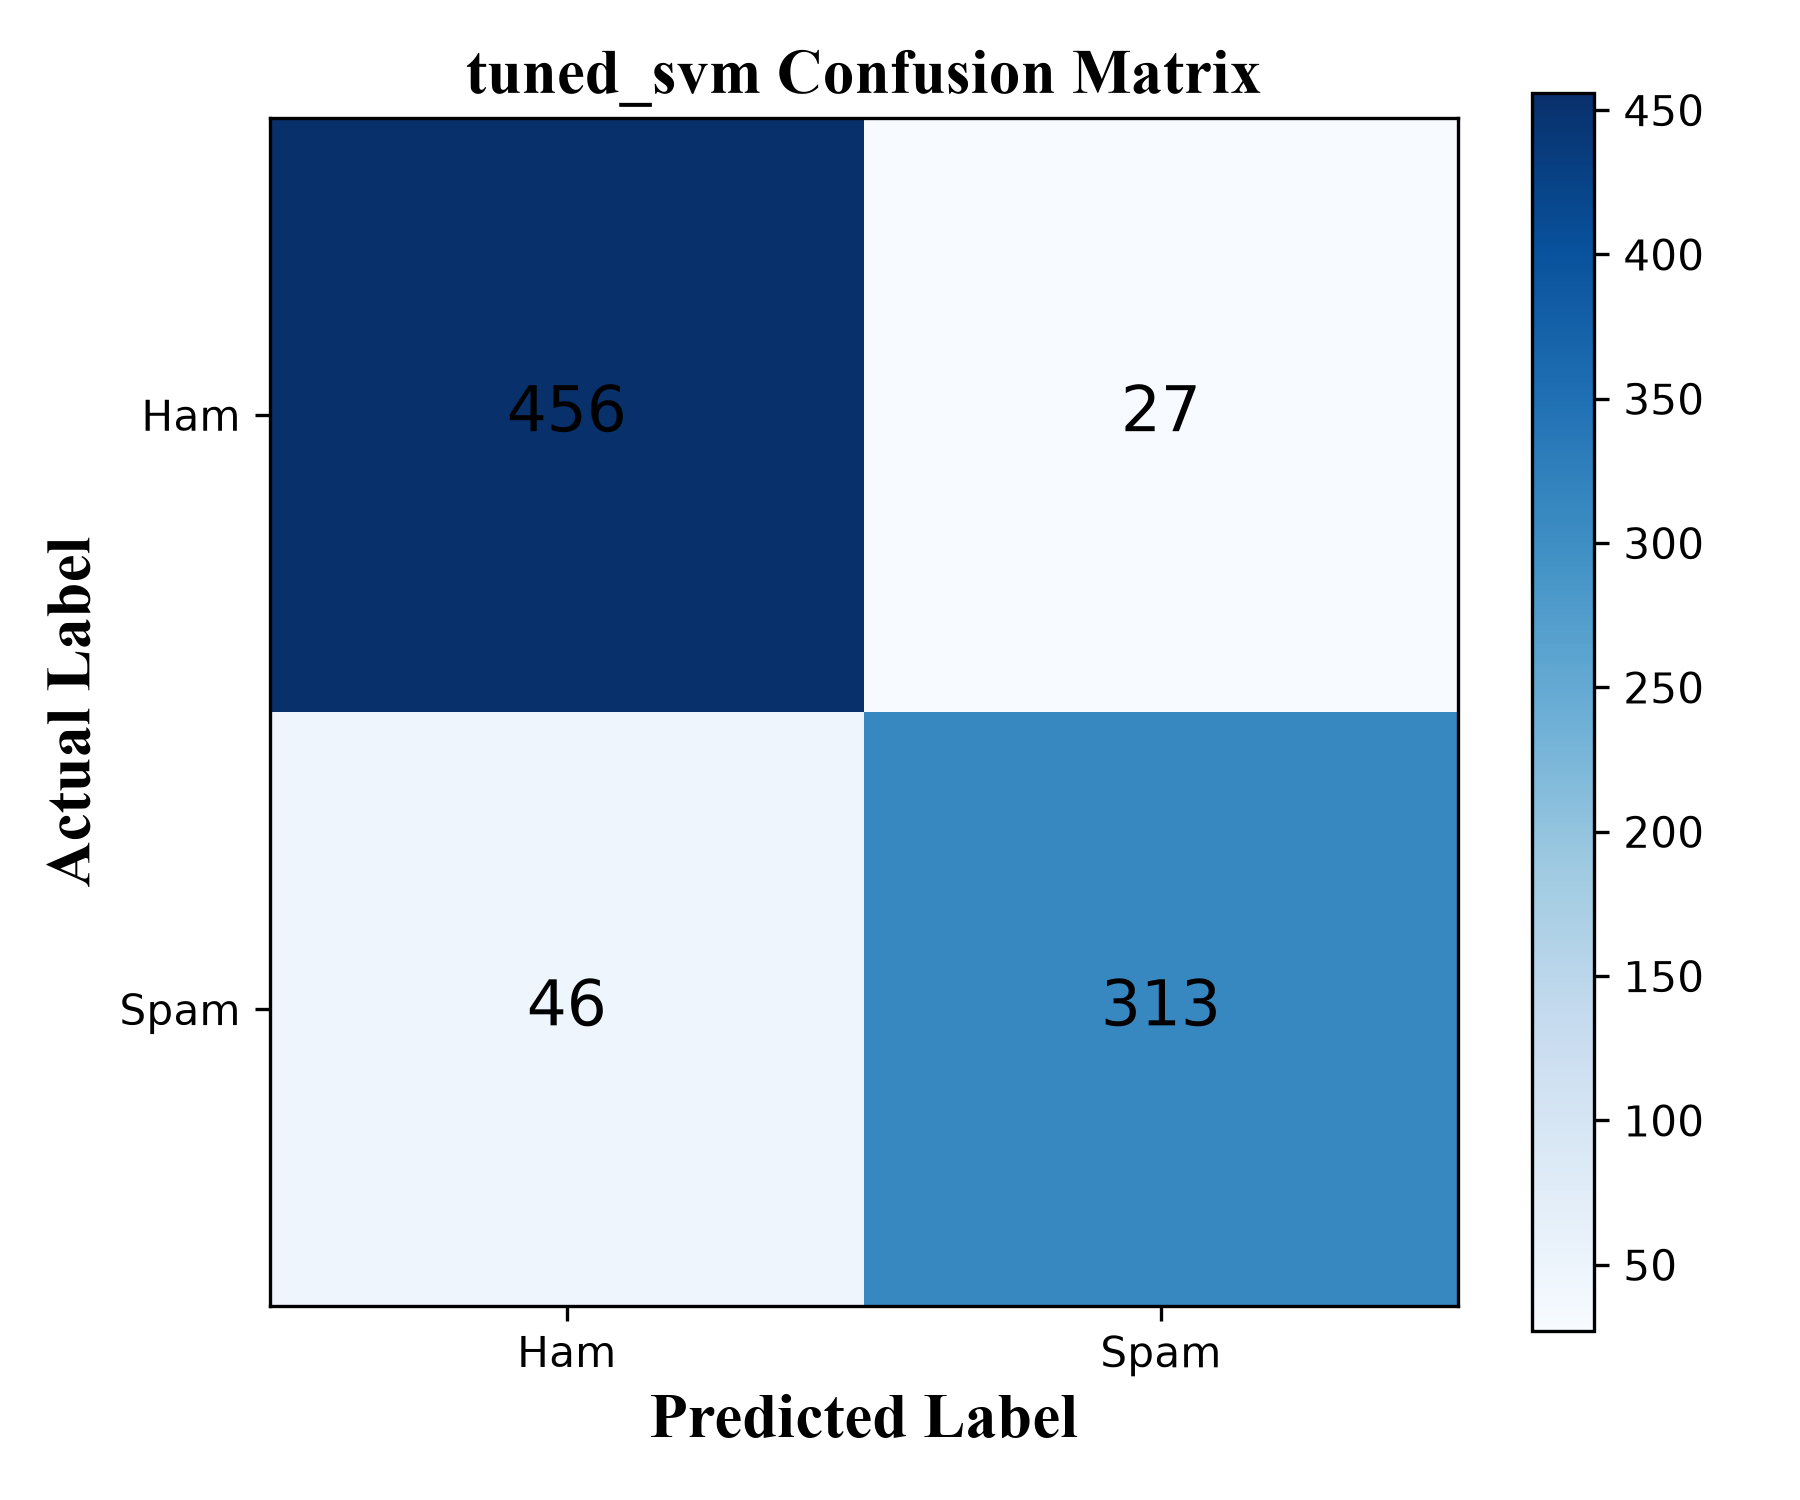
\includegraphics[width=0.55\linewidth]{tuned_svm_confusion_matrix.png}
\caption{Confusion Matrix -- Tuned SVM (RBF Kernel)}
\end{figure}

\textbf{Inference:} The tuned SVM achieves a test accuracy of 91.33\%, marginally lower than its own best cross-validation accuracy (92.99\%) and lower than the tuned Logistic Regression's test accuracy (92.04\%). This gap between CV and test performance is a mild indicator that the SVM's RBF kernel is somewhat more sensitive to the specific train/test split than the linear Logistic Regression model, though the difference is small enough to not indicate serious overfitting.

\section{Final Model Comparison}

\begin{table}[H]
\centering
\begin{tabular}{lrrrr}
\toprule
Model & Accuracy & Precision & Recall & F1-Score \\
\midrule
Logistic Regression & 0.9204 & 0.9320 & 0.8774 & 0.9039 \\
SVM & 0.9133 & 0.9206 & 0.8719 & 0.8956 \\
\bottomrule
\end{tabular}
\caption{Final Test Set Comparison -- Logistic Regression vs SVM}
\end{table}

\begin{figure}[H]
\centering
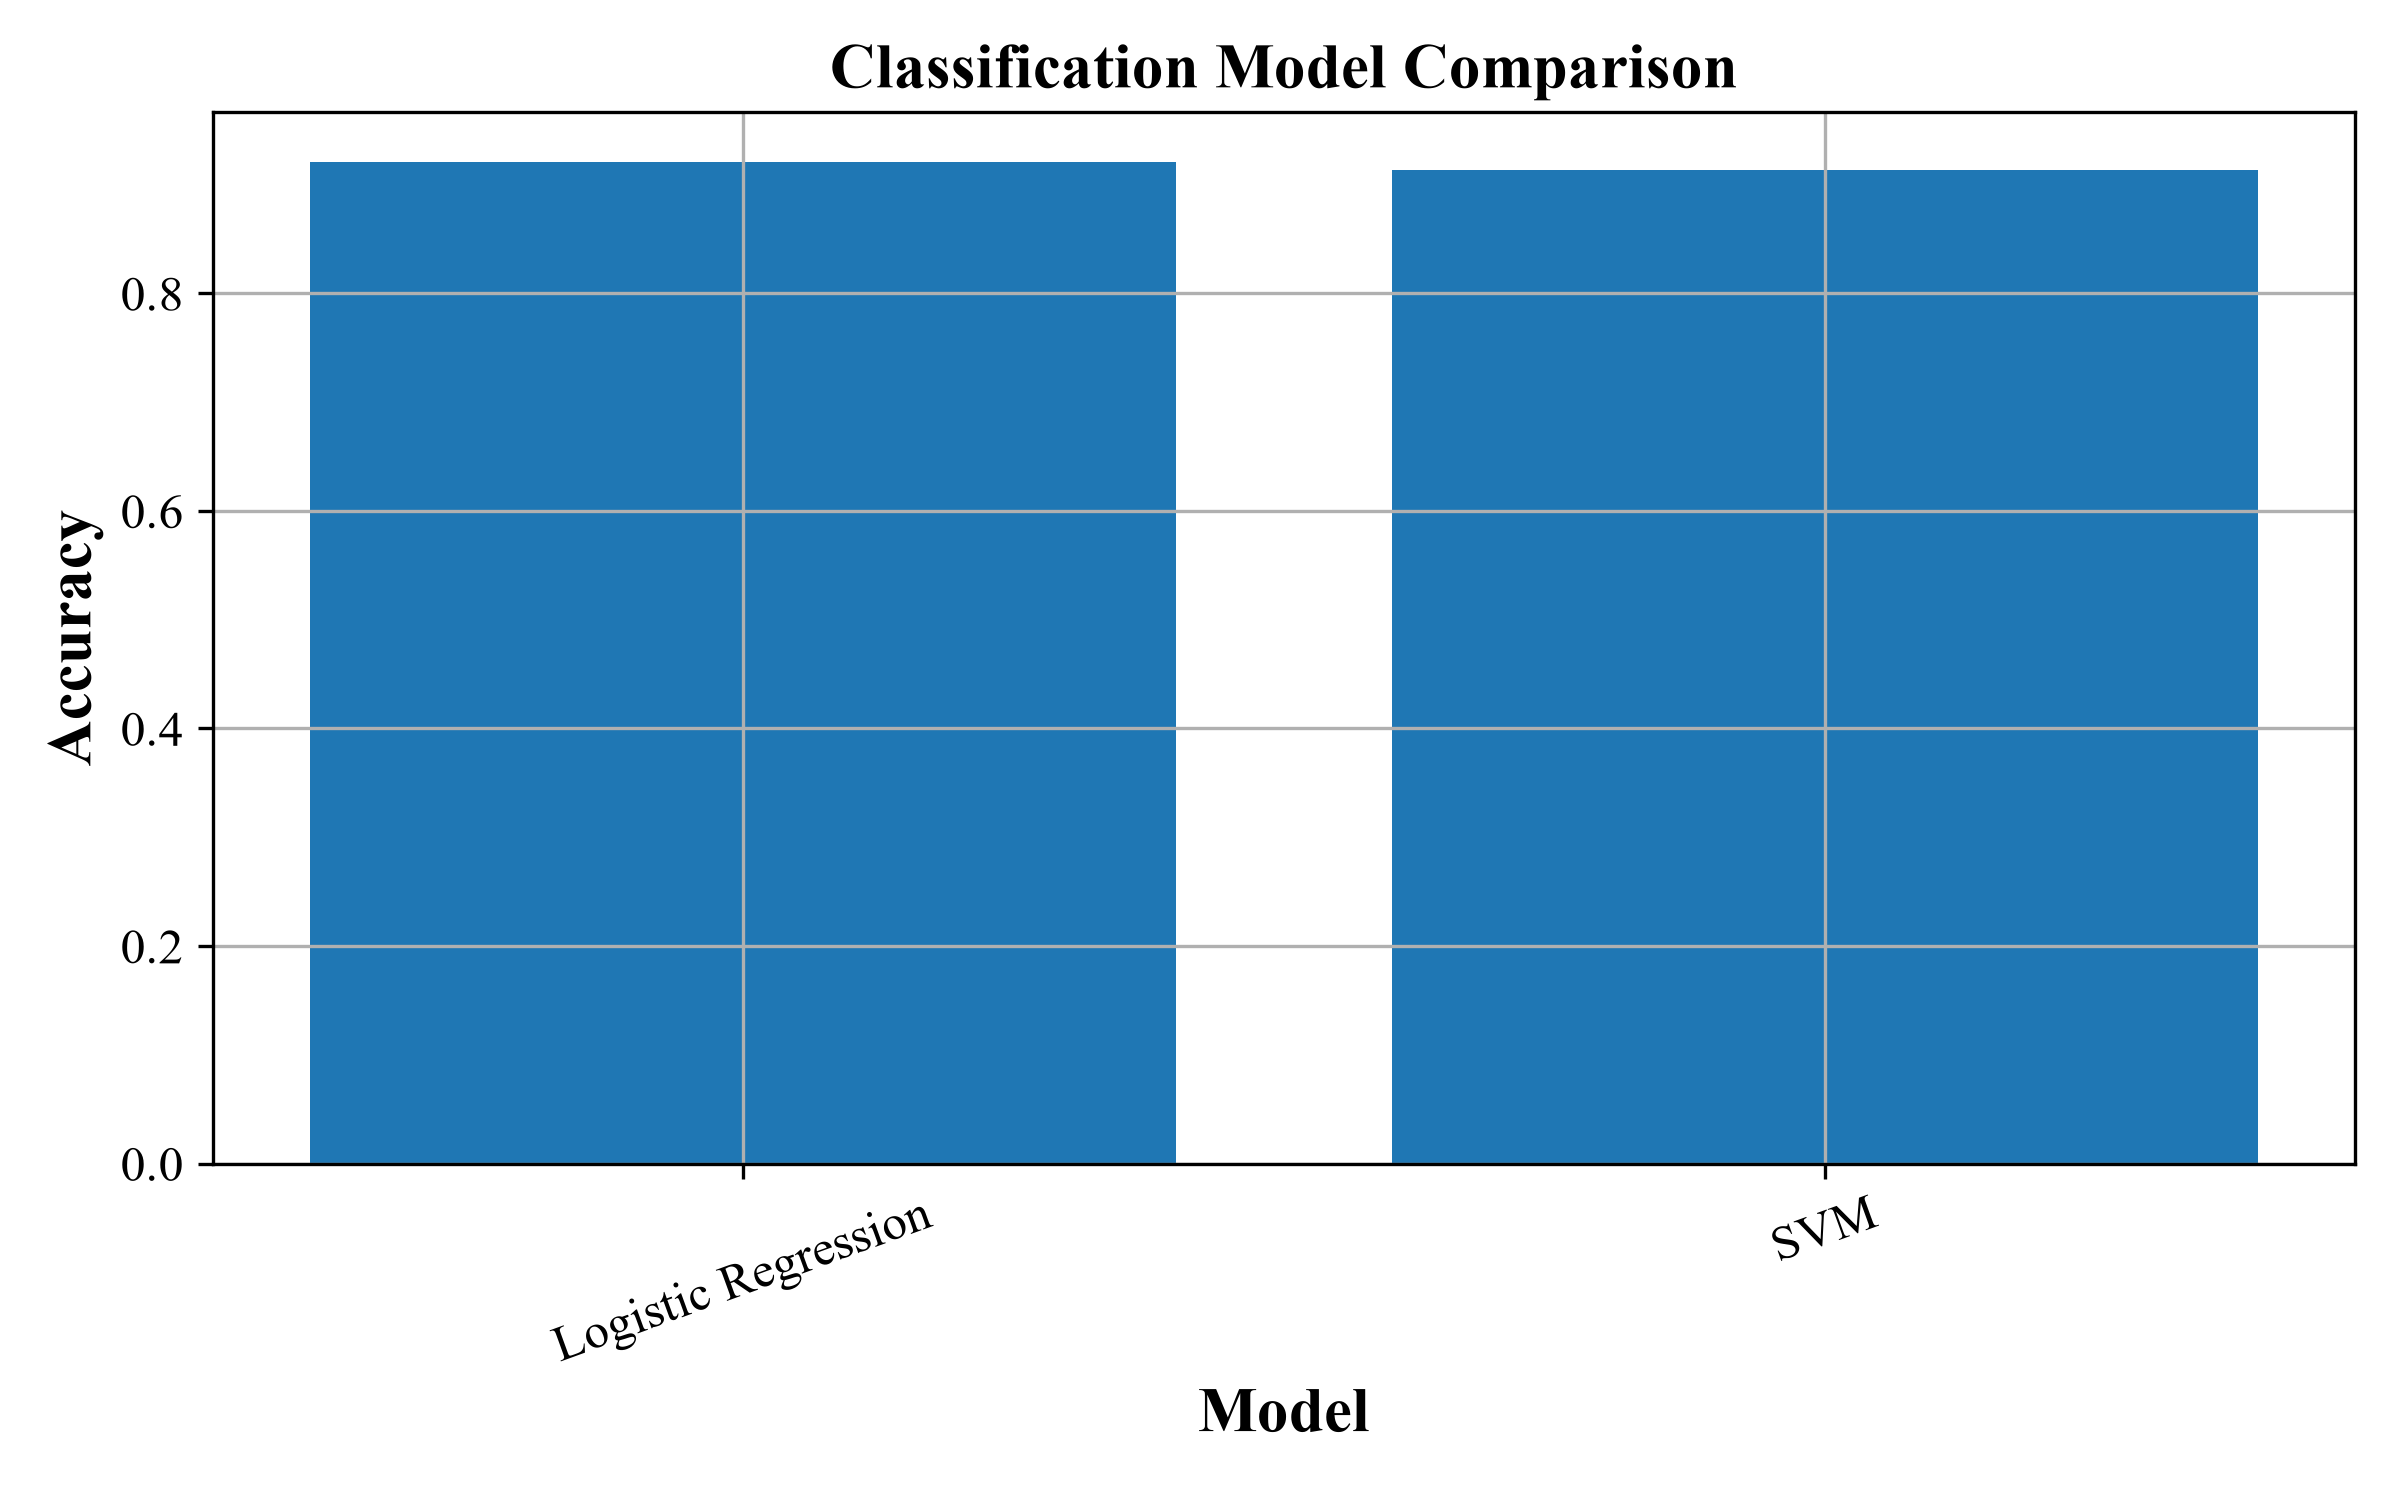
\includegraphics[width=0.7\linewidth]{classification_model_comparison.png}
\caption{Accuracy Comparison -- Logistic Regression vs SVM}
\end{figure}

\textbf{Inference:} Logistic Regression outperforms SVM across every reported metric on the held-out test set, though the margins are modest (approximately 0.7--0.9 percentage points). This suggests that, for the Spambase dataset in its standardized 57-feature form, the decision boundary is close enough to linear that a well-regularized linear model matches or exceeds a kernelized model, while remaining simpler and more interpretable.

\subsection*{Training and Prediction Time -- Final Models}

\begin{table}[H]
\centering
\begin{tabular}{lrr}
\toprule
Model & Training Time (s) & Prediction Time (s) \\
\midrule
SVM & 1.0410 & 0.0919 \\
Logistic Regression & 9.0465 & 0.0005 \\
\bottomrule
\end{tabular}
\caption{Training and Prediction Time -- Final Tuned Models}
\end{table}

\textbf{Inference:} Interestingly, the final tuned Logistic Regression model took considerably longer to train (9.05s) than SVM (1.04s), which is explained by the choice of the \texttt{saga} solver required for L1 regularization -- \texttt{saga} uses iterative stochastic averaging and converges more slowly than SVM's underlying quadratic solver for this dataset size. However, Logistic Regression's prediction time (0.0005s) is nearly 180$\times$ faster than SVM's (0.0919s), since SVM prediction requires computing kernel similarity against every stored support vector, while Logistic Regression prediction is a single dot-product operation. For a production spam filter that must classify large volumes of incoming email in real time, this makes Logistic Regression considerably more practical despite its longer one-time training cost.

\section{ROC Curve Analysis}

\begin{figure}[H]
\centering
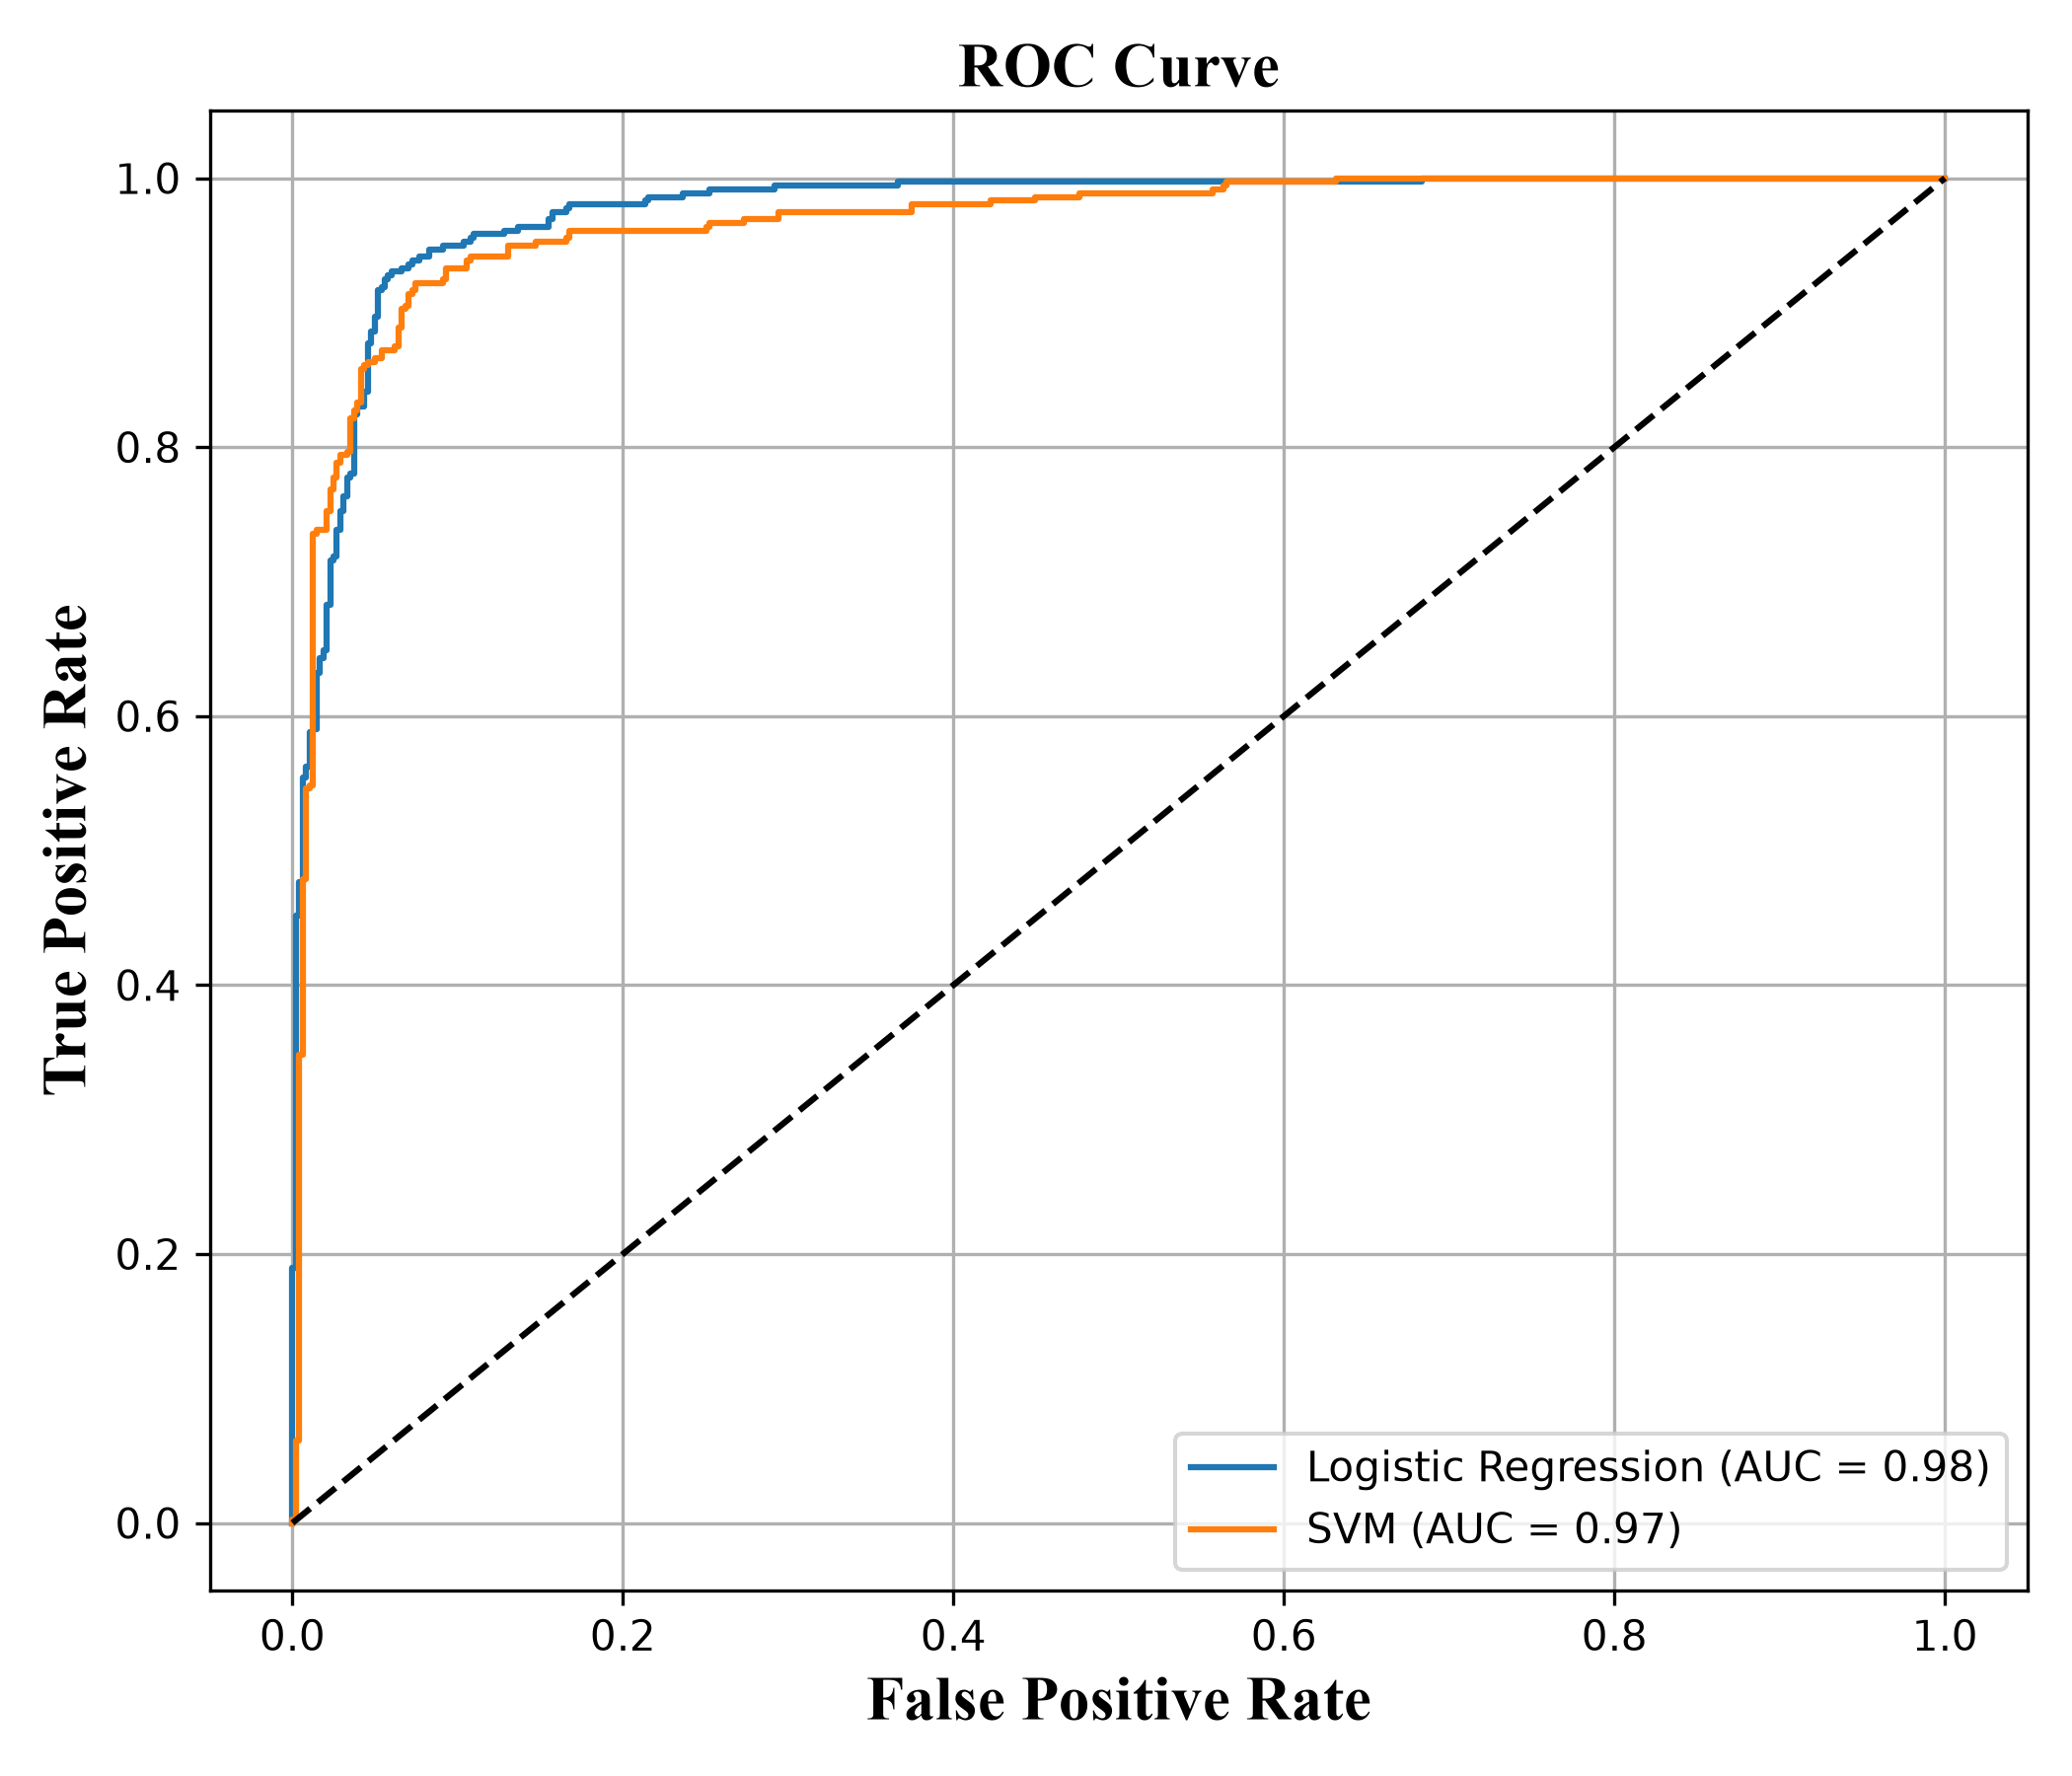
\includegraphics[width=0.65\linewidth]{roc_curve.png}
\caption{ROC Curve Comparison -- Logistic Regression vs SVM}
\end{figure}

\textbf{Inference:} The ROC curves for both models sit well above the diagonal (random-guess) line, confirming strong discriminative ability for both classifiers. The two curves are visually very close, consistent with the similar accuracy and F1-scores obtained on the test set. Both models achieve a high true positive rate at a low false positive rate, meaning that both can be tuned via classification threshold adjustment to prioritize either precision or recall depending on the operational cost of false positives (legitimate email marked as spam) versus false negatives (spam reaching the inbox).

\section{5-Fold Cross-Validation Results}

Cross-validation was performed on the full dataset (training + test combined) to obtain a more robust estimate of generalization performance independent of any single train-test split.

\begin{table}[H]
\centering
\begin{tabular}{lcc}
\toprule
Model & Average Accuracy & Std. Deviation \\
\midrule
Logistic Regression & 0.9230 & 0.0076 \\
SVM & 0.9261 & 0.0111 \\
\bottomrule
\end{tabular}
\caption{5-Fold Cross-Validation Performance (Full Dataset)}
\end{table}

\begin{figure}[H]
\centering
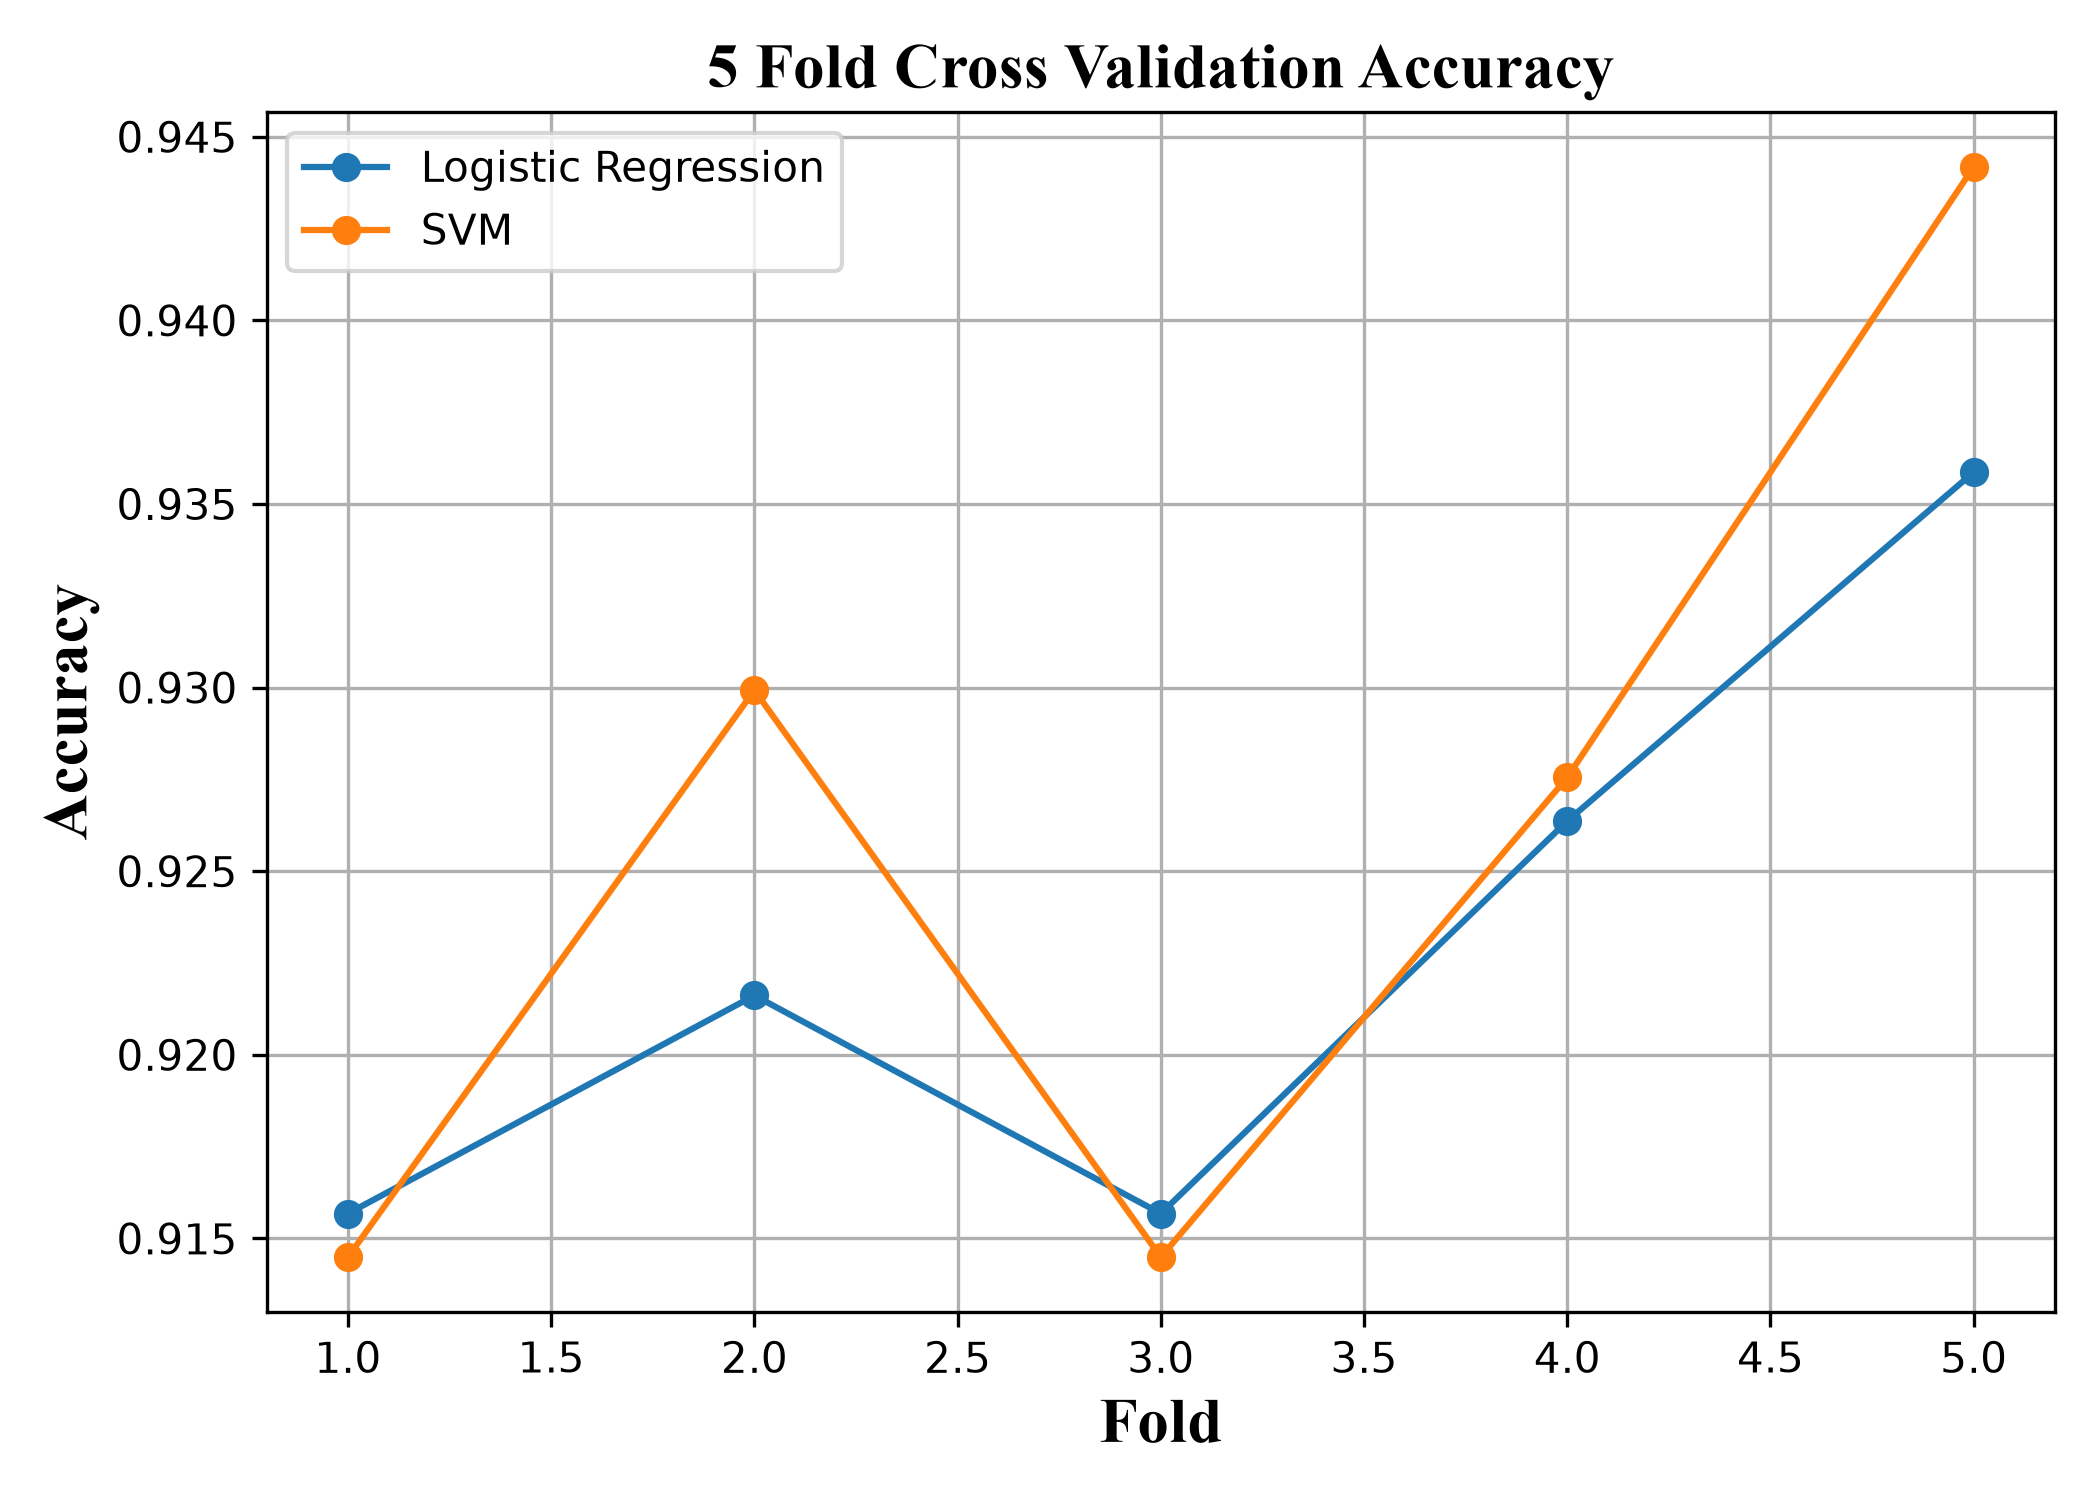
\includegraphics[width=0.7\linewidth]{classification_cv_scores.png}
\caption{5-Fold Cross-Validation Accuracy Scores by Fold}
\end{figure}

\textbf{Inference:} Under 5-fold cross-validation on the full dataset, SVM achieves a marginally higher average accuracy (92.61\%) than Logistic Regression (92.30\%), reversing the ranking seen on the single held-out test split. However, SVM's standard deviation across folds (0.0111) is roughly 46\% higher than Logistic Regression's (0.0076), indicating that SVM's performance is somewhat less consistent across different data partitions. This trade-off -- SVM's slightly higher average accuracy against Logistic Regression's greater stability -- is an important consideration: for a deployment setting where consistent, predictable performance is valued over a marginal accuracy gain, Logistic Regression's lower variance is a meaningful advantage.

\section{Discussion}

The experiment implemented and compared two fundamentally different classification approaches on the Spambase dataset. Logistic Regression, a linear probabilistic model, and SVM, evaluated across four kernels, were both trained and tuned using GridSearchCV with 5-fold cross-validation. The dataset itself required minimal preprocessing (only standardization, since it contains no missing values or categorical features), which allowed the experiment to focus primarily on model behavior and hyperparameter sensitivity.

The baseline kernel comparison revealed an important insight: the Polynomial kernel is highly sensitive to default hyperparameters and performed poorly (76.13\% accuracy) without tuning, while the Linear and RBF kernels performed strongly even at default settings, suggesting the true decision boundary for this dataset is close to linear. After tuning, Logistic Regression (L1, $C=100$) marginally outperformed the tuned SVM (RBF, $C=10$) on the held-out test set across all four metrics, though the reverse was true under 5-fold cross-validation on the full dataset, where SVM edged ahead in average accuracy but with higher variance.

From a deployment perspective, Logistic Regression offers three practical advantages: (1) near-instantaneous prediction time, critical for real-time email filtering at scale; (2) built-in interpretability via sparse L1 coefficients, allowing administrators to inspect which words/characters drive spam classification; and (3) lower variance in cross-validated performance. SVM's main advantage is a slightly higher theoretical ceiling on accuracy (as seen in CV), at the cost of substantially higher prediction latency and reduced interpretability.

A natural extension of this work would be to remove the 391 duplicate rows identified during EDA before splitting, to rule out any optimistic bias from near-identical samples appearing in both train and test partitions, and to explore ensemble methods (e.g. combining Logistic Regression and SVM via soft voting) to potentially capture the complementary strengths of both models.

\section{Conclusion}

This experiment successfully implemented and compared Logistic Regression and Support Vector Machine classifiers for binary spam detection on the Spambase dataset. Both models were tuned using GridSearchCV with 5-fold cross-validation, and evaluated using Accuracy, Precision, Recall, F1-Score, ROC-AUC, and cross-validation stability.

The tuned Logistic Regression model (L1 penalty, $C=100$, \texttt{saga} solver) achieved the best test-set performance, with 92.04\% accuracy and an F1-Score of 0.9039, narrowly outperforming the tuned SVM (RBF kernel, $C=10$, $\gamma=\text{scale}$), which achieved 91.33\% accuracy and an F1-Score of 0.8956. While 5-fold cross-validation on the full dataset showed SVM with a marginally higher average accuracy, its higher variance across folds and substantially slower prediction time make Logistic Regression the more practical and interpretable choice for this classification task. The experiment demonstrates that, for datasets with a largely linear decision boundary such as Spambase, well-regularized linear models can match or exceed kernel-based methods while offering superior efficiency and interpretability.

\section{References}

\begin{enumerate}
\item C. M. Bishop, \textit{Pattern Recognition and Machine Learning}, Springer, 2006.
\item T. Hastie, R. Tibshirani, and J. Friedman, \textit{The Elements of Statistical Learning}, 2nd ed., Springer, 2009.
\item S. Raschka and V. Mirjalili, \textit{Python Machine Learning}, 3rd ed., Packt Publishing, 2019.
\item F. Pedregosa et al., ``Scikit-learn: Machine Learning in Python,'' \textit{Journal of Machine Learning Research}, vol. 12, pp. 2825--2830, 2011.
\item M. Hopkins, E. Reeber, G. Forman, and J. Suermondt, ``Spambase Data Set,'' UCI Machine Learning Repository, 1999.
\item Scikit-learn Documentation, \url{https://scikit-learn.org/}
\end{enumerate}

\section*{Appendix}

\subsection*{A.1 Implementation Details}

The experiment was implemented using Python with reusable modules for:
\begin{itemize}
\item Data loading and inspection (\texttt{utils.py})
\item EDA (\texttt{eda.py})
\item Preprocessing pipeline (\texttt{preprocessing.py})
\item Classification model training (\texttt{classification.py})
\item Hyperparameter optimization (\texttt{hyperparameter.py})
\item Performance evaluation (\texttt{metrics.py})
\item Cross-validation (\texttt{validation.py})
\item Execution time benchmarking (\texttt{timing.py})
\item Visualization generation (\texttt{visualization.py})
\end{itemize}

\subsection*{A.2 Final Tuned Hyperparameters}

\begin{lstlisting}
Logistic Regression: {'C': 100, 'penalty': 'l1', 'solver': 'saga'}
SVM:                 {'C': 10, 'gamma': 'scale', 'kernel': 'rbf'}
\end{lstlisting}

\subsection*{A.3 Environment Activation Command}

\begin{lstlisting}
source /opt/anaconda3/bin/activate anaconda-navigation
\end{lstlisting}

\end{document}